\documentclass[pdflatex,sn-nature]{sn-jnl}

\usepackage{graphicx}
\usepackage{amsmath,amssymb,amsfonts}
\usepackage{booktabs}
\usepackage{xcolor}
\usepackage{float}
\usepackage{placeins}
\usepackage{url}
\usepackage{longtable,array}
\usepackage{calc}
\providecommand{\real}[1]{#1}
\providecommand{\tightlist}{}
\setlength{\LTcapwidth}{\textwidth}

%% --- pandoc compatibility block
\usepackage[normalem]{ulem}
\providecommand{\st}[1]{\sout{#1}}
\usepackage{textcomp}

% ======================================================================
% layout_tune.tex -- tune the sn-jnl text block + vertical density so the
% per-page content distribution reproduces the original revtex version.
% Reference revtex metrics: textwidth 468pt (164.5mm), textheight 665.5pt
% (234mm), baselineskip 21pt, font 12pt  ==>  ~70 chars/line, 31.7 lines/pg.
% sn-jnl uses a smaller body font, so width is scaled down to keep ~70
% chars/line, and \linespread loosens the leading to ~21pt to match lines/pg.
% ======================================================================

% --- horizontal: width scaled for sn-jnl's font; centred; no binding shift
\geometry{textwidth=152mm, textheight=236mm, top=24mm,
          hmarginratio=1:1, bindingoffset=0pt,
          marginparwidth=0pt, marginparsep=0pt}

% --- vertical leading (the main lever for lines-per-page); tuned empirically
% to ~21pt baselineskip, matching the revtex reference.
\linespread{1.74}

% --- float placement: the defaults reject any float taller than 70% of the
% text block, which defers the full-width multipanel figures to the end of the
% document. Loosen them so a figure can be placed in the section that cites it.
\renewcommand{\topfraction}{0.92}
\renewcommand{\bottomfraction}{0.85}
\renewcommand{\textfraction}{0.06}
\renewcommand{\floatpagefraction}{0.60}
\setcounter{topnumber}{2}
\setcounter{bottomnumber}{2}
\setcounter{totalnumber}{4}

% --- float / caption spacing; tight fig-to-caption gap (abovecaptionskip).
% Negative pulls the caption up to absorb trailing whitespace in the figures.
\setlength{\abovecaptionskip}{-4pt}
\setlength{\belowcaptionskip}{2pt}
\setlength{\textfloatsep}{12pt}
\setlength{\floatsep}{10pt}
\setlength{\intextsep}{10pt}

% --- last-resort stretch so unbreakable typewriter strings do not leave
% visibly loose lines; neither document carries an overfull box.
\setlength{\emergencystretch}{3em}

% --- tighten the reference list: sn-nature sets \bibsep=1em (a blank line
% between entries); reduce it so references sit close together.
\AtBeginDocument{\setlength{\bibsep}{1pt plus 0.3pt}}

% The loose body \linespread above would otherwise bleed into captions and
% stretch them. Reset captions to single spacing in a clean, sn-style caption
% (small font, bold run-in label, left-justified) -- NOT the squished 0.9.
\makeatletter
\long\def\@makecaption#1#2{%
  \vskip\abovecaptionskip
  \begingroup
    \small \linespread{1.0}\selectfont
    \leftskip\z@ \rightskip\z@ \parfillskip\z@ plus 1fil\relax
    \sbox\@tempboxa{\textbf{#1}\quad #2}%
    \ifdim \wd\@tempboxa >\hsize
      \textbf{#1}\quad #2\par
    \else
      \hb@xt@\hsize{\textbf{#1}\quad #2\hfil}%
    \fi
  \endgroup
  \vskip\belowcaptionskip}
\makeatother


%% the class loads hyperref itself with link colouring off. Re-assert at
%% egin{document} so that cross-references and citations are visibly clickable
\AtBeginDocument{\hypersetup{colorlinks=true,
  linkcolor={blue!55!black}, citecolor={blue!55!black},
  urlcolor={blue!55!black}, filecolor={blue!55!black},
  breaklinks=true, bookmarksnumbered=true, pdfstartview={FitH}}}

\newcommand{\rhoc}{\ensuremath{\rho}}
\newcommand{\fion}{\ensuremath{f_{\mathrm{i}}}}
\newcommand{\VM}{\ensuremath{E_{\mathrm{M}}}}

% --- Supplementary numbering: Section S1, Fig. S1, Table S1
\renewcommand{\thesection}{S\arabic{section}}
\renewcommand{\thefigure}{S\arabic{figure}}
\renewcommand{\thetable}{S\arabic{table}}
\renewcommand{\theequation}{S\arabic{equation}}

% --- the contents section-number box inherits 1.5em from the base class, too narrow
%     for two-digit numbers such as S15, so number and title collide. Widen only this
%     box; everything else stays as the base class sets it.
\makeatletter
\renewcommand*\l@section[2]{%
  \ifnum \c@tocdepth >\z@
    \addpenalty\@secpenalty
    \addvspace{1.0em \@plus\p@}%
    \setlength\@tempdima{2.8em}%
    \begingroup
      \parindent \z@ \rightskip \@pnumwidth
      \parfillskip -\@pnumwidth
      \leavevmode \bfseries
      \advance\leftskip\@tempdima
      \hskip -\leftskip
      #1\nobreak\hfil \nobreak\hb@xt@\@pnumwidth{\hss #2}\par
    \endgroup
  \fi}
\makeatother

% --- labels prefixed si-* so gen-si-xr.py can export them to the main text
\raggedbottom

\begin{document}

% \centering: the class Titlefont uses titraggedcenter, a "limited stretch" centring.
% Short lines (here the first) do not stretch enough and sit about 49 pt left of the
% rest. \centering restores full stretch, so every line is centred exactly.
\title[Supplementary Information]{\centering Supplementary Information for\\
Autonomous discovery of new structure-plausibility laws for explainable and rapid
crystal diagnosis and screening}

\author[1,2]{\fnm{Zhilong}\sur{Song}}

\author*[1,2,3]{\fnm{Lixue}\sur{Cheng}}\email{lixuecheng@ust.hk}

\affil[1]{\orgdiv{Department of Chemistry}, \orgname{Hong Kong University of Science
and Technology}, \orgaddress{\city{Kowloon}, \state{Hong Kong 999077},
\country{China}}}

\affil[2]{\orgdiv{IAS Center for AI for Scientific Discoveries}, \orgname{Hong Kong
University of Science and Technology}, \orgaddress{\city{Kowloon},
\state{Hong Kong 999077}, \country{China}}}

\affil[3]{\orgdiv{Department of Chemical and Biological Engineering}, \orgname{Hong
Kong University of Science and Technology}, \orgaddress{\city{Kowloon},
\state{Hong Kong 999077}, \country{China}}}

\abstract{This document provides the data sources and licences, definitions of all
measured quantities and laws, exact procedures used to damage structures, search and
testing procedures, and the full record of eleven refuted claims. It also documents
the data-split incident, reproduction instructions, additional tests of law accuracy
and physical meaning, the PRIS-derived synthesis score, and applications to generated
structures and database records.}

\maketitle

\makeatletter
\renewcommand*\l@subsection{\@dottedtocline{2}{1.5em}{3.4em}}
\makeatother
\tableofcontents
\clearpage

\section{Autonomous discovery protocol and its audit trail}\label{note:s1}

\subsection{What was autonomous}\label{s1.1-what-was-autonomous}

Hypotheses, feature designs, experiments, diagnostics and refutations were generated
and executed by AI agents across multiple sessions. The models used across the numbered investigations are recorded in the public session
archive.
No detailed scientific hypothesis was supplied by a human. The agents operated in a
shell with read/write access to the datasets. The programme ran under one continuous analysis protocol across sessions between
2026-07-27 and 2026-08-14, comprising 568 numbered investigations and four final
analyses whose plans were recorded before evaluation (pre-registered analyses). Human
input set the broad goal of finding improved crystal-structure laws and formulas,
redirected the scope, and provided authorisation
decisions on whether to use the reserve data that had been kept out of law development.

\subsection{How the discovery trail was audited}\label{s1.2-the-audit-trail}

Unlike a conventional study, the scientific decision trail is recoverable from
publicly auditable records:

{\def\LTcaptype{none} % do not increment counter
\begin{longtable}[]{@{}
  >{\raggedright\arraybackslash}p{(\linewidth - 2\tabcolsep) * \real{0.5000}}
  >{\raggedright\arraybackslash}p{(\linewidth - 2\tabcolsep) * \real{0.5000}}@{}}
\toprule\noalign{}
\begin{minipage}[b]{\linewidth}\raggedright
Artefact
\end{minipage} & \begin{minipage}[b]{\linewidth}\raggedright
Content
\end{minipage} \\
\midrule\noalign{}
\endhead
\bottomrule\noalign{}
\endlastfoot
Raw session archive (JSONL, 6,381 records) & timestamped user and assistant messages, tool calls and returned results. The public evidence export excludes hidden reasoning, encrypted content and system or developer records \\
\texttt{git\ log} & code state at each milestone, including the \texttt{prereg-v1.0} and \texttt{stage2-complete} tags \\
Script docstrings (60 files, 15,360 lines) & each script's header records \emph{why} it was written, what it replaced, and which earlier conclusion it falsified \\
Workflow transcripts (14 runs) & parallel research and independent checking agents, with their individual results \\
\end{longtable}
}

\textbf{The eleven refuted claims in Supplementary Fig.~\ref{sifig:ledger} are
verifiable from preserved records rather than asserted retrospectively.} Each claim
has a timestamp, the code that produced it, the code that falsified it, and the
document revision in which it was withdrawn.

\subsection{Scale and outcomes of the autonomous search}\label{s1.3-run-statistics}

The statistics below cover the entire programme described above, under the
same data conventions and automated checks. Source records for every session are
preserved in the repository record.

{\def\LTcaptype{none} % do not increment counter
\begin{longtable}[]{@{}
  >{\raggedright\arraybackslash}p{(\linewidth - 2\tabcolsep) * \real{0.5000}}
  >{\raggedright\arraybackslash}p{(\linewidth - 2\tabcolsep) * \real{0.5000}}@{}}
\toprule\noalign{}
\begin{minipage}[b]{\linewidth}\raggedright
Metric
\end{minipage} & \begin{minipage}[b]{\linewidth}\raggedright
Value
\end{minipage} \\
\midrule\noalign{}
\endhead
\bottomrule\noalign{}
\endlastfoot
Wall-clock span & 2026-07-27 10:31 $\rightarrow$ 2026-08-14 \\
Investigations and final analyses & 572 (568 numbered rounds + 4 pre-registered analyses on held-out data) \\
Candidate evaluations across the broader autonomous programme, documented lower bound & 2,037,606 (scope stated below) \\
Analysis scripts written & 615 (60 + 546 + 9) with 575 accompanying test files and 317 plans fixed before analysis \\
Feature tables and archived outputs & 84 parquet tables (1.4\,GB) + 72,583 result files (34.9\,GB) \\
Structures analysed in the structure-law programme & 99,162 experimental + 5.95\,M Alexandria + 2.03\,M ELEMENTA. The final analyses newly featurised 42,691 structures \\
PU/PSS analysis pool & The separate PU analysis pool is documented in Section S16 \\
Tool invocations, initial session & 1,095 (Bash 806, Read 110, Edit 56, Write 35), plus 14 multi-agent workflows and 41 literature queries \\
Conclusions stated and then self-refuted & 11 \\
Prespecified outcome and constraints for Set~4 & Met: all pre-registered satisfaction and damage-detection criteria \\
Prespecified outcome and constraints for PSS & Met: decision-rate and structural-baseline criteria; held-out DFT comparison reported separately \\
Evidence retained here & 8 retained laws (Law~1--Law~8) and PSS \\
\end{longtable}
}

The retained laws and the fitted score have distinct roles. Law~1--Law~8 are the
physicochemical laws, and Set~4 met every pre-registered success criterion. PSS is the
task-specific continuous ranking layer developed from the same structural space.

\textbf{Plotting conventions of main-text Fig.~1e.} One mark denotes one
investigation that reached its own verdict. The four lanes contain investigations that met
a success criterion, missed a success criterion, showed no gain, or were abandoned.
No mark is shown for 175 investigations that produced no verdict. Of these, 131
could not run because inputs or preceding steps were unavailable, 37 had no
archived verdict that could be checked, and 7 measured quantities without testing
a success criterion. Investigations on adjacent screening problems are excluded
from the strip. The optimal-tree analysis was evaluated only on the discovery
split, so it appears as a no-gain marker rather than on the held-out curve.

\textbf{Itemisation of the candidate count.} The documented lower bound of
2,037,606 counts hypotheses across both the crystal-law problem and adjacent
screening problems in the same programme. It sums only search sizes stated
explicitly in archived round reports, where each contribution remains traceable.
Search grids without a recorded size are excluded, so the true total is larger.
This programme-wide count is distinct from the 8{,}466 candidate laws evaluated
in the final Set~4 analysis. More than 99.9 per cent of documented candidates were
removed before confirmation by a search plan fixed in advance or by predefined
inclusion checks. Nearly all candidates that reached confirmation then failed
criteria for replication, transfer to other data, or robustness across
multiple settings.

\subsection{The audit catches documented errors, not unknown ones}\label{s1.4-a-caveat-on-what-this-does-and-does-not-demonstrate}

The audit demonstrates that AI agents can conduct a multi-day empirical programme
in which later checks detect errors produced within the same workflow. Each of the
eleven documented failures was detected only after its claim had entered the report
as a result. \textbf{We have no estimate of the number of undetected errors.} The
absence of the relevant diagnostic allowed each false conclusion to survive.
This omission motivated the checklist in Supplementary Fig.~\ref{sifig:ledger}.

\begin{figure}[!htbp]
  \centering
  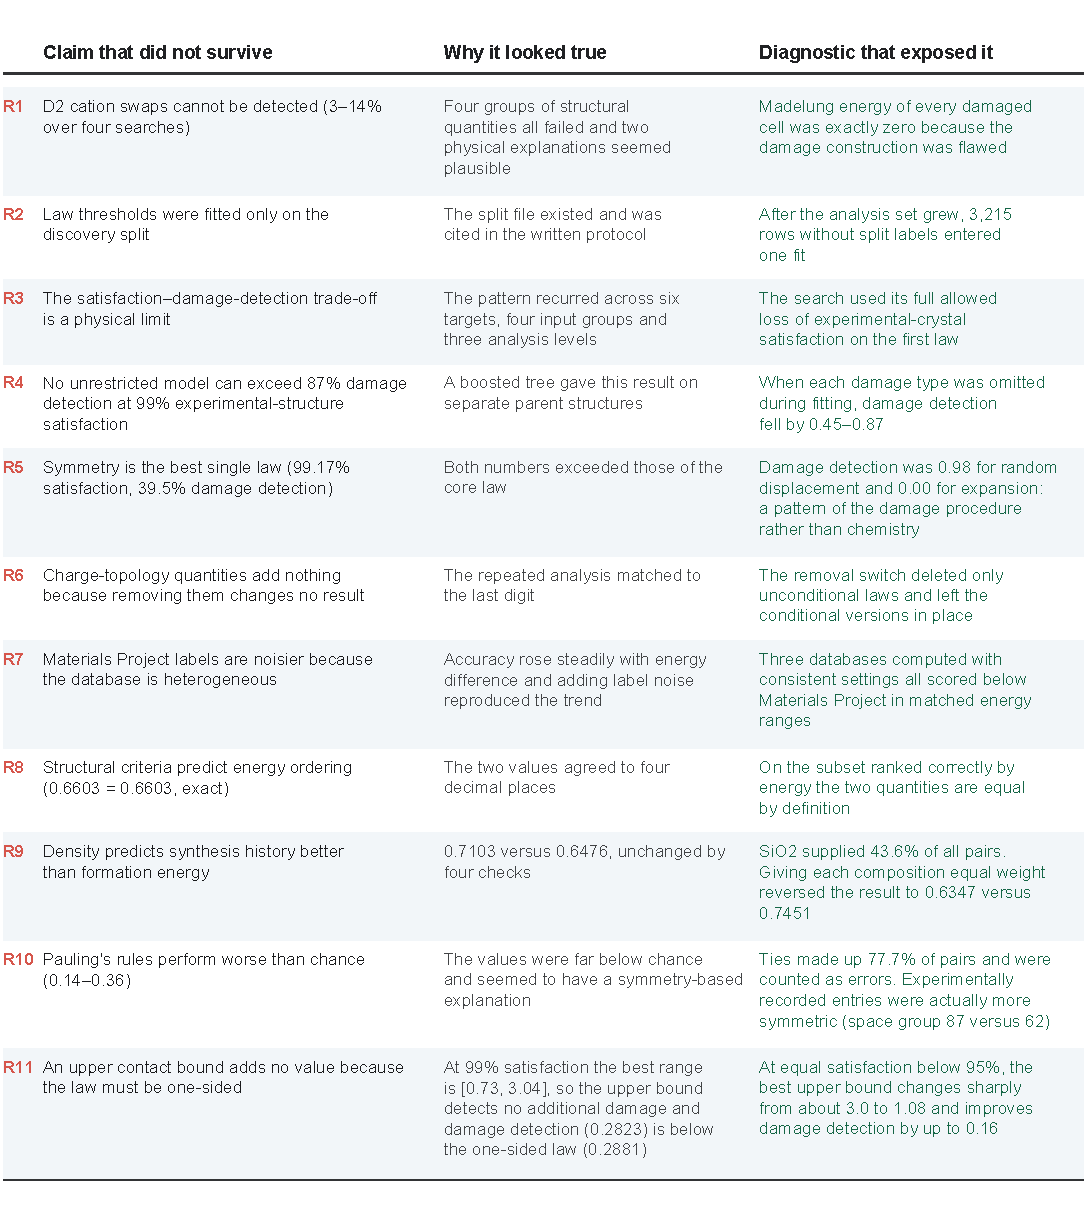
\includegraphics[width=\textwidth]{figs/figS1_refutation_ledger.pdf}
  \caption[Refuted-claim ledger]{\textbf{Refuted-claim ledger.} Each row lists a claim
  identifier used throughout the Supplementary Information. The three text columns record
  the withdrawn claim, the evidence or reasoning that initially supported it, and the
  diagnostic that exposed the error. Alternating grey shading separates entries, while red
  identifiers and green diagnostic text distinguish the audit fields.}
  \label{sifig:ledger}
\end{figure}

\begin{figure}[!htbp]
  \centering
  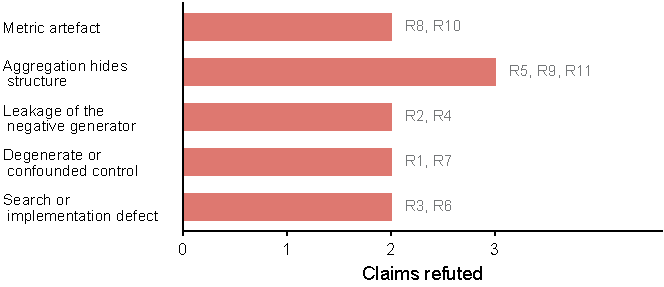
\includegraphics[width=0.68\textwidth]{figs/figS2_failure_modes.pdf}
  \caption[Refutations grouped by failure mode]{\textbf{Refutations grouped by failure
  mode.} Each audited claim from Supplementary Fig.~\ref{sifig:ledger} is assigned once to
  the diagnostic category that exposed it. Categories are arranged on the vertical axis,
  horizontal bar length gives the number of assigned claims, and R identifiers at the bar
  ends link each category to the corresponding ledger entries.}
  \label{sifig:modes}
\end{figure}

\clearpage
\section{Data sources, licences and the analysis set}\label{note:s2}

\subsection{Sources}\label{s2.1-sources}

{\def\LTcaptype{none} % do not increment counter
\begin{longtable}[]{@{}
  >{\raggedright\arraybackslash}p{(\linewidth - 6\tabcolsep) * \real{0.2500}}
  >{\raggedright\arraybackslash}p{(\linewidth - 6\tabcolsep) * \real{0.2500}}
  >{\raggedright\arraybackslash}p{(\linewidth - 6\tabcolsep) * \real{0.2500}}
  >{\raggedright\arraybackslash}p{(\linewidth - 6\tabcolsep) * \real{0.2500}}@{}}
\toprule\noalign{}
\begin{minipage}[b]{\linewidth}\raggedright
Source
\end{minipage} & \begin{minipage}[b]{\linewidth}\raggedright
Records
\end{minipage} & \begin{minipage}[b]{\linewidth}\raggedright
Use
\end{minipage} & \begin{minipage}[b]{\linewidth}\raggedright
Licence
\end{minipage} \\
\midrule\noalign{}
\endhead
\bottomrule\noalign{}
\endlastfoot
ICSD & 73,823 & experimental structures & FIZ Karlsruhe, \textbf{not redistributable} \\
COD & 25,339 & experimental structures & CC0 \\
Materials Project & 154,377 & energies, ICSD linkage, experimental records & CC-BY-4.0 \\
Alexandria PBE-3D & 5,952,515 & polymorph ranking, consistent settings & CC-BY-4.0 \\
ELEMENTA (core) & 2,028,008 trajectory endpoints & polymorph ranking, \texttt{max\_force} available & CC-BY-NC-4.0 \\
LeMat candidate pool & 108,580 & polymorph ranking & mixed \\
OMat24 & \emph{screened out} & --- & see S2.3 \\
\end{longtable}
}

\subsection{How structures entered the analysis}\label{s2.2-the-analysis-funnel}

The analysis began with 99,162 experimental structures. Excluding unary
structures, for which Pauling's rules are undefined, left 98,352. Of the full
cohort, \textbf{35,490 structures (35.8\%)} had both assignable formal charges and
every required feature. Formal-charge assignment alone covers 64.5\%, as
\S{}S2.4 explains.

\subsection{Why OMat24 was screened out}\label{s2.3-why-omat24-was-screened-out}

OMat24's training partition consists of AIMD snapshots at 1000 K and 3000 K and rattled
configurations, which are non-equilibrium structures intended for
interatomic-potential training.
Energy differences there reflect thermal excursion, not phase stability. The
\texttt{rattled-relax} partition does contain optimisations, but its records are
\textbf{trajectory frames}. A sample of 8,001 records spanned 334 trajectories.
Complete trajectories contain 24 frames, but the row-level sample ended partway through one
trajectory. Retaining only the endpoints left
more than one endpoint for just \textbf{2 of 332 compositions}. The partition
therefore cannot form polymorph groups.

\subsection{Formal-charge assignment limits the evaluable population}\label{s2.4-the-64-that-cannot-be-judged}

No charge-balanced integer valence assignment could be found for 41.1\% of 523
sampled held-out structures. The table below partitions these failures; its
denominator is the subset without an assignment.

{\def\LTcaptype{none} % do not increment counter
\begin{longtable}[]{@{}
  >{\raggedright\arraybackslash}p{(\linewidth - 2\tabcolsep) * \real{0.5000}}
  >{\raggedright\arraybackslash}p{(\linewidth - 2\tabcolsep) * \real{0.5000}}@{}}
\toprule\noalign{}
\begin{minipage}[b]{\linewidth}\raggedright
Cause
\end{minipage} & \begin{minipage}[b]{\linewidth}\raggedright
Share of failures
\end{minipage} \\
\midrule\noalign{}
\endhead
\bottomrule\noalign{}
\endlastfoot
Mixed-valence transition metals (resolvable with non-integer mean valence) & \textbf{72.1\%} \\
No variable-valence element: integer combinations genuinely unsolvable & 27.9\% \\
\end{longtable}
}

The primary Law~1--Law~8 analysis uses integer assignments. Charge-assignment
coverage is the fraction of structures with assigned formal charges. In a
separate analysis, a non-integer mean-valence fallback raised this coverage from
64.5\% to \textbf{80.9\%}. The retained laws and thresholds were applied without
refitting. The four-law core was satisfied by 0.9256 of the newly admitted
population, compared with 0.9577 of the integer-valence population (121 groups,
95\% CI $\approx$ $\pm$4.7 pp).

\section{Feature definitions}\label{note:s3}

We used pymatgen \texttt{CrystalNN(\allowbreak weighted\_cn=False,\allowbreak\
x\_diff\_weight=0)} to identify neighbours. Valences came from
composition-derived formal charges. We \textbf{never used \texttt{BVAnalyzer}},
because inferring valence from bond lengths before testing bond-valence laws is
circular.

For the common-denominator comparison in main-text Fig.~2c, each Pauling
criterion produced one Boolean verdict for each of 5{,}297 held-out structures:
(1) mean rule-2 bond-strength deviation at most 0.01; (2) rule-3 edge-or-face
sharing fraction at most 0.10; (3) no rule-4 high-valence violation; and (4)
satisfaction of rule 5. Under the benchmark convention also used for PRIS, an
unavailable measurement counts as satisfying the criterion. Experimental-structure
satisfaction is the fraction satisfying the law set under this convention. The
four rules were satisfied by 2{,}312, 598, 2{,}279 and 4{,}325 structures,
respectively, and 345 satisfied all four. The separate historical audit retains
each rule's natural site-orbit, orbit-pair or structure unit and is not used in
Fig.~2c.

The feature tiers distinguish composition-only inputs (T0), low-cost structural
inputs (T1), and quantities that require a fully specified structure (T3).

{\def\LTcaptype{none} % do not increment counter
\begin{longtable}[]{@{}
  >{\raggedright\arraybackslash}p{(\linewidth - 4\tabcolsep) * \real{0.21}}
  >{\raggedright\arraybackslash}p{(\linewidth - 4\tabcolsep) * \real{0.70}}
  >{\raggedright\arraybackslash}p{(\linewidth - 4\tabcolsep) * \real{0.09}}@{}}
\toprule\noalign{}
\begin{minipage}[b]{\linewidth}\raggedright
Symbol
\end{minipage} & \begin{minipage}[b]{\linewidth}\raggedright
Definition
\end{minipage} & \begin{minipage}[b]{\linewidth}\raggedright
Tier
\end{minipage} \\
\midrule\noalign{}
\endhead
\bottomrule\noalign{}
\endlastfoot
\texttt{bl\_min} & min over cation--anion bonds of \emph{d} / {[}\emph{r}(cat) + \emph{r}(an){]}, Shannon radii by (element, oxidation state, CN) & T3 \\
\texttt{bl\_mean} & same ratio, averaged over all cation--anion bonds & T3 \\
\texttt{mad\_max} & maximum site Madelung energy from an Ewald sum with formal charges & T3 \\
\texttt{madz\_range} & range of (site Madelung energy $\div$ absolute formal-charge magnitude), scale-free across chemistries & T3 \\
\texttt{min\_opp\_frac} & min over ions of (fraction of its neighbours with opposite charge) & \textbf{T1} \\
\texttt{frac\_like\_bonds} & fraction of all bonds joining same-sign ions & \textbf{T1} \\
\texttt{econ\_mean/max} & Hoppe effective coordination number, \emph{w} = exp{[}1 $-$ (\emph{d}/\emph{d}min)$^6${]} & T3 \\
\texttt{mef\_mean} & Hoppe MEFIR effective-radius mismatch, signed & T3 \\
\texttt{aa\_min/mean} & ligand--ligand contact ratio, the geometric core of Pauling's first rule & T3 \\
\texttt{ecc\_max} & \textbar $\Sigma$ \textbf{\^u}$_i$\textbar{} / \emph{n}, off-centring of the cation in its coordination shell & T3 \\
\texttt{p5\_n\_distinct} & mean number of distinct CN values per (element, oxidation state) & T1 \\
\texttt{fi} & Pauling ionicity 1 $-$ exp($-$0.25 $\Delta$$\chi$$^2$) & \textbf{T0} \\
\end{longtable}
}

\textbf{T3 quantities require an existing structure and cannot be calculated
from composition alone.} They are appropriate here because this work evaluates
existing structures.

\subsection{Oxidation states}\label{s3.1-oxidation-states}

For the PRIS analysis, \texttt{discriminate.guess\_oxi} assigns formal oxidation states
from composition alone by integer charge balancing. Native CIF oxidation-state
annotations are not used. \texttt{BVAnalyzer} was never called anywhere in the pipeline,
for the reason above. Structures for which no charge-balanced integer assignment can be
found are retained with missing charge values. Deleting them would select
against mixed-valence chemistry, which contains the most information about
bond-valence laws. Missing values therefore remain missing and are handled by
the convention in \S{}\ref{s3.3-missing-values} rather than being imputed.

\subsection{Fixed radius and bond-valence lookups make parameter choices reproducible}
\label{s3.1b-lookup}

Every contact ratio and valence sum follows one fixed parameter-lookup sequence.
\emph{Shannon radii} are keyed by (element, oxidation
state, coordination number). When the optional charge-assignment fallback of Section S2.4 is
used, its non-integer mean valence is rounded to the nearest integer before lookup, with its sign
retained. If the observed coordination number has no tabulated entry, the lookup
tries CN, CN$-$1, CN$+$1 and then VI, in that order. If none is available for
the element and oxidation state, it uses a representative per-element ionic
radius. The final fallback is 1.0\,\AA{} for a cation and 1.4\,\AA{} for an
anion. Spin-split Shannon entries are resolved
through the same coordination fallback, so the radius used for a 3d ion is
spin-agnostic. We did not separately quantify sensitivity to high-spin versus
low-spin radii.

\emph{Bond-valence parameters} come from the IUCr \texttt{bvparm2020}
compilation. They are keyed by cation element and integer valence, and by anion
element and integer valence. For each pair, the lookup takes the first-listed
parameter set and its tabulated $b$, never a generic constant. Pairs without
tabulated parameters are skipped and counted. Every bond-valence statistic
reports the fraction of neighbour entries with available parameters
(\texttt{bv\_param\_cov}). A structure-level Law~8 value is emitted only when
the structure contains at least two parameterised cation--anion neighbour
entries. Its mean deviation includes all non-zero-charge sites and is normalised
by the formal charge.

\subsection{Neighbour-algorithm robustness}\label{s3.2-neighbour-algorithm-robustness}

CrystalNN is the primary neighbour algorithm. For robustness, we recomputed
BrunnerNN and MinimumDistanceNN on a common random subsample of 3{,}000
structures (\texttt{random\_state=7}). The comparison quantifies the sensitivity
of Law~1 and the individual Pauling criteria. The exact spreads, in percentage points, were
0.18 for $\rhoc{} \geq 0.735$, 5.74 for Pauling's fourth rule,
4.05 for the first, 3.93 for the third, 1.81 for the fifth and 0.83 for the
second. Thus the contact-ratio criterion was 32-fold less sensitive than the
most fragile criterion within this algorithm family. Because all three
algorithms share pymatgen's tolerance conventions, the 0.18-percentage-point
spread brackets disagreement within that family of definitions.

\subsection{Missing values and minimum feature availability}\label{s3.3-missing-values}

A missing feature value counts as satisfying a law for benchmark calculations. Only features computable
on more than 0.9 of experimental structures are therefore admitted to the search. This prevents a criterion
from receiving high satisfaction merely because values are unavailable. When applied to a new
structure, a missing charge or required feature produces no verdict and routes the structure
to review.

\section{Searching for simple crystal-plausibility laws}\label{note:s4}

\subsection{The search balances satisfaction against damage detection}\label{s4.1-objective}

Here, satisfaction is the fraction of experimental structures that satisfy a law set under
the missing-value convention above. Damage detection is the fraction of damaged
structures that fail it.

The candidate model is a set of \emph{N} single-feature threshold laws joined by
AND. Its objective is to maximise damage detection on composition-matched damaged
structures. Experimental-structure satisfaction must remain above a stated
minimum. An optional second constraint requires every chemical group's
satisfaction to exceed the same stated group minimum.

\subsection{Executable checks exposed two search defects}\label{s4.2-two-defects-found-in-our-own-search}

\textbf{(a) The greedy step used the entire allowed loss in satisfaction.} Beam
search ranked candidates only by damage detection. At depth 1, it therefore
selected a law whose satisfaction was exactly at the required minimum, leaving
no room for another law. At a required satisfaction of 0.99, this produced a
single-law set. The complete repair allocates half the beam to candidates ranked
by \emph{damage detection gained per unit reduction in satisfaction}. The other
half remains ranked by total damage detection plus the weakest class's rate.
Damage detection at a required satisfaction of 0.95 rose from
0.658 to 0.734.

\textbf{(b) Ban-filter failure and correction.} Conditional laws use the
composite key \texttt{"G:\textless{}guard\textgreater{}:\textless{}target\textgreater{}"}.
Filtering only on the plain column name therefore removed unconditional variants
but left conditional variants in the search. Several feature-removal tests
reported as ``identical after removal'' although they had removed nothing.
The defect is recorded as R6 in Supplementary Fig.~\ref{sifig:ledger}, and the corrected
ablation is summarised in Section~\ref{note:s7}.

\subsection{A fixed search grid limits how much the search can adapt to the data}\label{s4.3-search-configuration}

A candidate law is a (feature, direction, percentile-threshold) triple. Each law
set can contain at most one threshold per feature column. Conditional laws take
the form ``if $G$ then $T$'' and are evaluated as $\neg G \vee T$. The guard
$G$ is restricted to T0 and T1 selectors, so it never requires the metric
structure that the law judges. Beam search maximises damage detection subject to
minimum overall satisfaction and, optionally, minimum satisfaction for each
anion group.

All values in this subsection are from the discovery split. At a required
satisfaction of 0.99, the search returned five laws with satisfaction 0.9917 and
damage detection 0.304. At 0.98, it returned three laws with satisfaction 0.9813
and damage detection 0.4161. At the recommended value of 0.95, it returned five
laws with satisfaction 0.9539, damage detection 0.6224, and weakest-group
satisfaction 0.928. This operating-point sequence uses the repaired allocation
described above, not a further refinement. Beam width, minimum gain per added
law, and the percentile grid are fixed in the search implementation.

\subsection{Composition controls prevent misleading cross-database comparisons}\label{s4.4-scoring-formulas}

Structure counts, accessible energy spans and the concentration of pairs in one
composition differ strongly among ranking databases. We therefore report the source
populations and repeat the comparison inside a common hull-energy window
(Supplementary Fig.~\ref{sifig:ranking-data}a,b). Every accuracy is first computed
within a composition and then averaged with equal weight across compositions. This
prevents a database with many near-duplicate pairs from dominating the comparison and
separates dataset composition from the structural signal being tested.

\begin{figure}[!htbp]
  \centering
  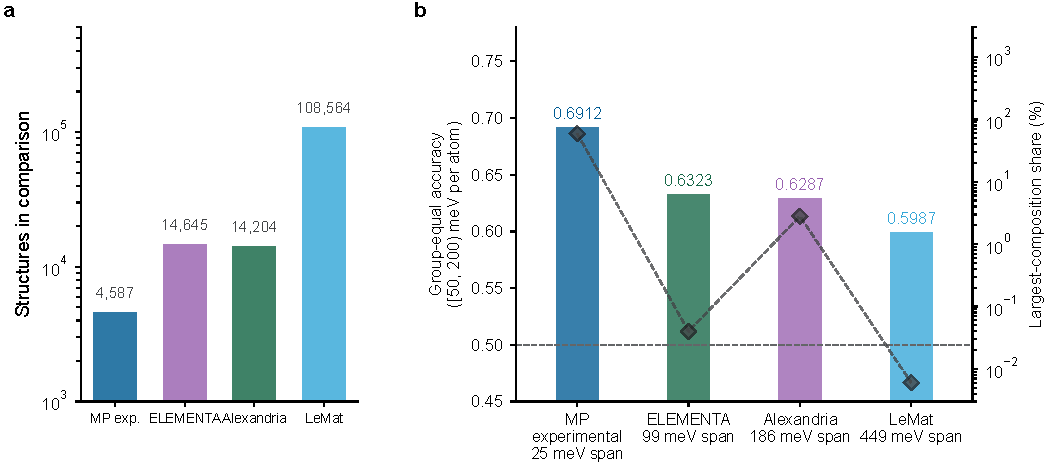
\includegraphics[width=\textwidth]{figs/figS3_ranking_data.pdf}
  \caption[Ranking-data scale and composition]{\textbf{Ranking-data scale, energy-span
  matching and composition concentration.}
  \textbf{a},~Database-specific structure counts on a logarithmic vertical axis. Labels
  above the bars give the counts, and colours identify the source databases.
  \textbf{b},~Composition-group-equal ranking accuracy within the common
  hull-energy window. Bars report accuracy on the left axis. Diamonds and a
  dashed line report the largest composition's pair share on the logarithmic
  right axis. Horizontal-axis sublabels give the intra-composition energy spans.
  The horizontal dashed line marks chance accuracy.}
  \label{sifig:ranking-data}
\end{figure}

\section{Composition-preserving perturbations isolate structural failure modes}\label{note:s5}

Five damage types, each preserving composition, stoichiometry and atom count, were retained.
Here, $\Delta E_{\mathrm{M}}$ is the change in Madelung energy relative to the experimental
parent:

{\def\LTcaptype{none} % do not increment counter
\begin{longtable}[]{@{}
  >{\raggedright\arraybackslash}p{(\linewidth - 8\tabcolsep) * \real{0.2000}}
  >{\raggedright\arraybackslash}p{(\linewidth - 8\tabcolsep) * \real{0.2000}}
  >{\raggedright\arraybackslash}p{(\linewidth - 8\tabcolsep) * \real{0.2000}}
  >{\raggedright\arraybackslash}p{(\linewidth - 8\tabcolsep) * \real{0.2000}}
  >{\raggedright\arraybackslash}p{(\linewidth - 8\tabcolsep) * \real{0.2000}}@{}}
\toprule\noalign{}
\begin{minipage}[b]{\linewidth}\raggedright
Class
\end{minipage} & \begin{minipage}[b]{\linewidth}\raggedright
Operation
\end{minipage} & \begin{minipage}[b]{\linewidth}\raggedright
Median $\Delta E_{\mathrm{M}}$ (eV per atom)
\end{minipage} & \begin{minipage}[b]{\linewidth}\raggedright
Median \texttt{bl\_min}
\end{minipage} & \begin{minipage}[b]{\linewidth}\raggedright
Verdict
\end{minipage} \\
\midrule\noalign{}
\endhead
\bottomrule\noalign{}
\endlastfoot
--- & (experimental structures) & --- & 0.937 & --- \\
D1 & uniaxial compression 15--30\% & \textbf{$-$2.100} & 0.791 & retained, flagged \\
D2 & cation--cation swap (formal charges must differ) & +0.929 & 0.814 & valid \\
D3 & random displacement 0.3--0.8 \AA{} & +0.090 & 0.521 & valid \\
D4 & isotropic expansion 20--40\% & +6.278 & 1.234 & valid \\
D5 & cation--anion swap & \textbf{+5.803} & \textbf{0.930} & valid despite being geometrically invisible \\
\st{S6} & \st{shear strain 10--25\%} & $-$0.004 & 0.881 & \textbf{discarded} \\
\end{longtable}
}

\textbf{D1 is flagged} because its Madelung energy \emph{decreases}: compression
shortens cation--anion distances and increases Coulomb attraction. Pauling's
electrostatic framework contains no short-range repulsion. The supplementary
\texttt{bl\_min} measure supplies this missing contact term and identifies the
compressed structures as unreasonable.

\textbf{S6 was discarded} because neither independent probe confirmed it as
unfavourable. Its median $\Delta E_{\mathrm{M}}$ was $-0.004$ eV per atom, and only
10\% of cases fell below the \texttt{bl\_min} threshold. These independent
energetic and geometric probes therefore did not support retaining S6. Doing so
would have repeated the unverified-damage design failure exposed by R1, the D2
cation-swap implementation error described in Section S12.

\textbf{D5 is the informative damage type.} Geometrically, it is nearly
indistinguishable from experimental structures (\texttt{bl\_min} 0.930 versus
0.937). Electrostatistically, it is catastrophic. No bond-length criterion
detects it well (damage detection 0.03--0.21). The audited Law~6 like-charge ban
closes this blind spot. Adding Law~6 to the four-law core raises held-out D5
damage detection from 0.262 to 0.576, a gain of 0.314. The largest gain on any
other class is 0.057.
The complete damage-type comparison on the discovery and held-out splits is shown in
Supplementary Fig.~\ref{sifig:perclass}.

\begin{figure}[!htbp]
  \centering
  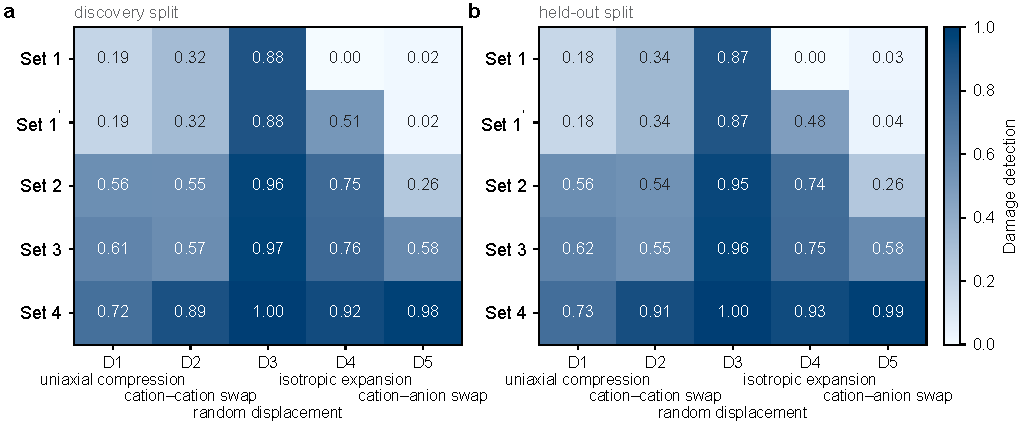
\includegraphics[width=\textwidth]{figs/figS4_perclass.pdf}
  \caption[Per-class damage detection]{\textbf{Damage detection by perturbation class
  on the discovery and held-out splits.} \textbf{a},~Discovery split used for law
  selection. \textbf{b},~Held-out split evaluated with the law sets fixed. Rows are PRIS
  law sets and columns are the D1--D5 composition-preserving perturbations. Cell colour
  and printed text encode the within-class damage-detection fraction on a shared scale,
  and the column labels define the perturbation operations.}
  \label{sifig:perclass}
\end{figure}

\begin{figure}[!htbp]
  \centering
  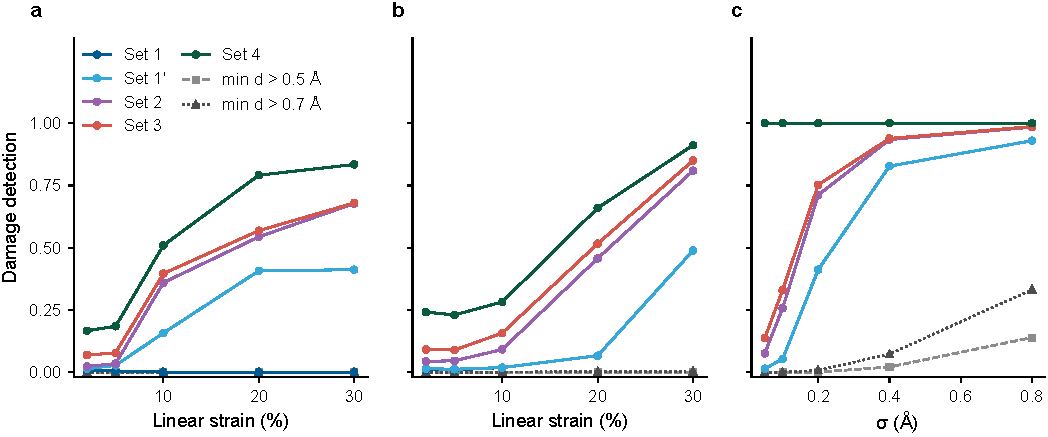
\includegraphics[width=\textwidth]{figs/figS5_amplitude_response.pdf}
  \caption[Damage detection versus perturbation amplitude]{\textbf{Damage detection
  versus perturbation amplitude.} All panels use the same fixed parent-structure cohort,
  with the vertical axis giving the fraction of perturbed structures detected.
  \textbf{a},~Isotropic expansion. \textbf{b},~Uniaxial compression.
  \textbf{c},~Gaussian displacement. Solid lines with circles identify PRIS law sets,
  while dashed lines with squares and dotted lines with triangles identify the two
  minimum-distance criteria.}
  \label{sifig:amplitude}
\end{figure}

\section{The eleven refuted conclusions}\label{note:s6}

Supplementary Fig.~\ref{sifig:ledger} provides an overview of all eleven
refutations, including why each claim was initially persuasive and which
diagnostic exposed it. Supplementary Fig.~\ref{sifig:modes} groups the same
events by the diagnostic failure mode that exposed them. The accompanying
machine-readable ledger
preserves the complete trace for every event. Two cases deserve extended
treatment below.

\subsection{R8: an identity mistaken for evidence}\label{s6.1-r8-an-identity-mistaken-for-evidence}

We observed that a structural score's accuracy on the energy-correct subset
equalled its sign agreement with energy to four decimal places (0.6603 = 0.6603).
We initially interpreted this identity as evidence that the score predicted
energy ordering.

On that subset, \emph{y} = $\mathbb{1}${[}$-$$\Delta$E \textgreater{} 0{]} by construction, so

accuracy = mean($\mathbb{1}${[}s\textgreater0{]} = \emph{y}) = mean($\mathbb{1}${[}s\textgreater0{]} = $\mathbb{1}${[}$-$$\Delta$E\textgreater0{]}) = sign-agreement.

Recomputing across eight criteria gave differences of exactly +0.0000 in all eight cases.
\textbf{A four-decimal agreement that holds for every criterion is a definition, not a finding.}

\subsection{R10: a lesson recorded, then repeated}\label{s6.2-r10-a-lesson-recorded-then-repeated}

Supplementary Section~\ref{note:s13} requires tie and error rates to be reported
separately. Pauling's fifth rule illustrates why: it yields a non-tied comparison
for only 0.2230 of pairs and ties in 88.4\% of composition groups. Its accuracy
therefore changes substantially when ties are credited, excluded, or counted as
errors. The later synthesis-target analysis nevertheless counted 77.7\% ties as
errors. This scoring error produced the claim that Pauling's rules perform worse
than chance (0.14--0.36). The proposed symmetry mechanism was also refuted:
experimentally recorded entries are \emph{more} symmetric, with medians of 87
versus 62.

\textbf{Recording a lesson does not ensure that it is applied.} The corrected diagnostics are now
automated checks in the pipeline, not only statements in the document.

\section{Which feature families improve damage detection}\label{note:s7}

The table reports each feature family's marginal contribution to law-set damage
detection at minimum satisfaction 0.95 on five discovery-split damage types.

{\def\LTcaptype{none} % do not increment counter
\begin{longtable}[]{@{}
  >{\raggedright\arraybackslash}p{(\linewidth - 4\tabcolsep) * \real{0.40}}
  >{\raggedright\arraybackslash}p{(\linewidth - 4\tabcolsep) * \real{0.20}}
  >{\raggedright\arraybackslash}p{(\linewidth - 4\tabcolsep) * \real{0.40}}@{}}
\toprule\noalign{}
\begin{minipage}[b]{\linewidth}\raggedright
Family added
\end{minipage} & \begin{minipage}[b]{\linewidth}\raggedright
Damage detection
\end{minipage} & \begin{minipage}[b]{\linewidth}\raggedright
Increment
\end{minipage} \\
\midrule\noalign{}
\endhead
\bottomrule\noalign{}
\endlastfoot
Coordination statistics + Pauling quantities (baseline) & 0.509 & --- \\*
\textbf{+ Shannon-radius bond ratios} & \textbf{0.734} (four types) & \textbf{+22.5 pp} \\*
+ electrostatics / Madelung & 0.6224 (five types) & \texttt{mad\_max} enters, forced by D5 \\*
+ charge topology & 0.6224 & \textbf{0} (two independent lines of evidence) \\*
+ angular (\texttt{ecc}, \texttt{angvar}) & 0.6254 & \textbf{0} \\*
+ symmetry & --- & \textbf{excluded}, see R5 \\
\end{longtable}
}

The values 0.734 and 0.6224 are not directly comparable because the former covers four
damage types whereas the latter includes D5. Shannon-radius bond ratios provide the largest
gain on the first four types, while adding D5 brings the electrostatic \texttt{mad\_max}
feature into the selected set.

\section{Split discipline, revisions and the reserve split-labelling error}\label{note:s8}

The pre-registration is preserved at git tag \texttt{prereg-v1.0} and commit
\texttt{ec4b464}. Seed 20260728 assigned structures to three partitions:
discovery (22,925), held-out (9,634), and sealed reserve (5,748). Assignment used
a seeded hash of each structure identifier rather than composition. Structures
sharing a composition can therefore cross partitions.
The resulting discovery-to-held-out changes in satisfaction and damage detection are
shown overall in Supplementary Fig.~\ref{sifig:split-consistency} and by damage type in
Supplementary Fig.~\ref{sifig:perclass}.

\textbf{Revision R1} corrected the design-effect measurement. \textbf{Revision
R2} corrected the recorded source of oxidation-state assignments. Both were
committed as \texttt{da563b1} \textbf{after} the analysis plan was fixed, and
their timestamps are disclosed here.

\textbf{The reserve split-labelling error.} After the plan was fixed, the
analysis set was widened to all experimental structures. Newly admitted rows had
no split label. A full-sample percentile-threshold fit consequently included
3,215 reserve rows in the law analysis and 863 in the historical formula fit.
An \texttt{assert\_clean()} check now refuses to fit if any row lacks a split label
or belongs to the reserve. \textbf{Because reserve rows influenced this
threshold fit, the reserve can no longer serve as a fully independent final
test.}

\textbf{The first authorised evaluation of the reserve.} Explicit authorisation
opened the reserve on 2026-08-01 (opening index 1), using one of three permitted
evaluations. The analysis tested V4, a candidate five-law refinement that adds
an integer-valence condition to the like-charge ban. Its success criteria were
fixed before evaluation. Overall damage detection had to increase by $+0.02$,
or detection in the weakest damage type by $+0.03$, while satisfaction could
change by no less than $-0.005$.

The reserve contained 3,163 evaluable experimental structures and 2,195 damaged
structures. V4 changed satisfaction by $-0.0003$, overall damage detection by
$+0.0105$, and detection in the weakest baseline class, D1 uniaxial compression, by
$-0.0102$. Thus satisfaction remained within its limit, but neither performance
alternative met its gate. D5 detection nevertheless increased by $+0.182$ as an additional
class-specific result. V4 is therefore refuted at its stated effect size and does not
appear in the main text.

Two findings extend beyond V4. First, the integer-valence condition behaved as
intended on reserve data. Without it, nitride-group satisfaction fell by 5.8
percentage points; the condition recovered all but 0.7 percentage points. This
confirms fractional-valence polyanions as the natural exception to a
like-charge-contact law. Second, the effect size was $+0.0238$ on the repeatedly
reused held-out split and $+0.0355$ on post-2019 data, but only $+0.0105$ on the
reserve. This is the project's direct measurement of effect inflation after
repeated held-out use. It also shows that a time-separated dataset cannot replace
an untouched reserve. Two permitted evaluations remain.

\begin{figure}[!htbp]
  \centering
  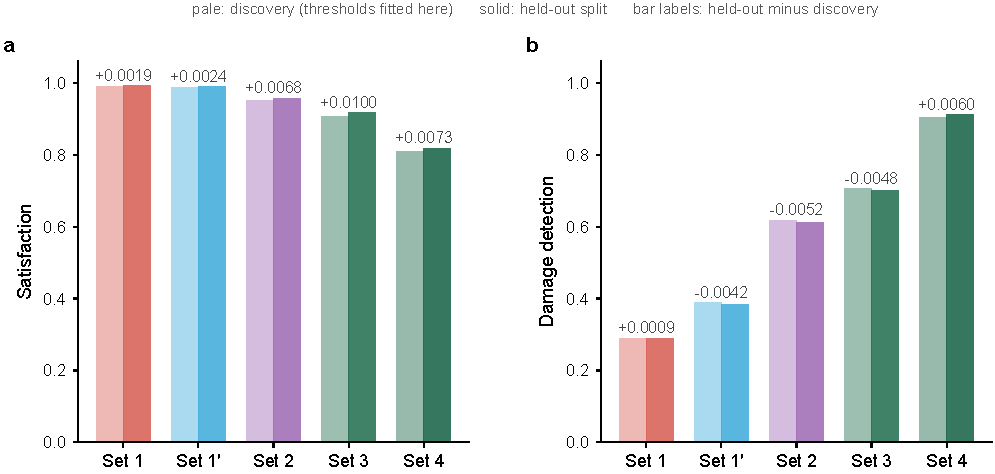
\includegraphics[width=\textwidth]{figs/figS6_split_consistency.pdf}
  \caption[Discovery and held-out splits]{\textbf{PRIS law sets on the discovery and
  held-out splits.} \textbf{a},~Fraction of experimental structures satisfying each
  law set. \textbf{b},~Fraction of damaged structures detected, pooled across
  perturbation classes. Pale bars show the discovery partition used to select the
  thresholds, and solid bars show held-out evaluation without refitting. Labels above
  paired bars report the held-out value minus the discovery value, and both panels use
  the same fractional scale.}
  \label{sifig:split-consistency}
\end{figure}

\textbf{Composition-unseen sensitivity.} Because the structure-identifier hash permits
composition overlap, we performed an additional outcome-blind subgroup analysis using only
the discovery and held-out partitions. Reduced formulas defined composition groups, and
each chemically damaged structure inherited the reduced composition of its experimental
parent. The PRIS laws, thresholds and missing-feature convention remained frozen. Of
5{,}297 held-out experimental structures, 3{,}631 (68.55\%) shared a reduced composition
with discovery and 1{,}666 (31.45\%) did not; the corresponding counts among 3{,}612 damaged
structures were 2{,}406 and 1{,}206. Confidence intervals used 10{,}000 percentile-bootstrap
resamples of whole reduced-composition clusters (seed 20260829).

For Set~4, experimental-structure satisfaction was 81.38\% (95\% interval,
79.73--82.99\%) for composition-shared structures and 82.71\% (80.65--84.67\%) for
composition-unseen structures; damage detection was 90.73\% (89.53--91.92\%) and 91.87\%
(90.28--93.42\%), respectively (Supplementary Fig.~\ref{sifig:pris-composition-holdout}).
Weighting reduced compositions equally gave 82.04\% satisfaction and 91.64\% detection in
the unseen subgroup. A stricter subset whose exact element sets were absent from discovery
retained 83.17\% satisfaction among 1{,}046 experimental structures and 91.49\% detection
among 799 damaged structures. Bond-valence coverage was lower in the composition-unseen
subgroup (83.25\% for experimental and 81.01\% for damaged structures) than in the shared
subgroup (85.90\% and 89.24\%); counting an unavailable value as satisfying a law can raise
satisfaction but cannot inflate damage detection. This analysis is a sensitivity test
within the existing held-out partition, not a newly collected external holdout; ``chemical
system'' denotes the exact element set rather than a broader chemical family.

\begin{figure}[!htbp]
  \centering
  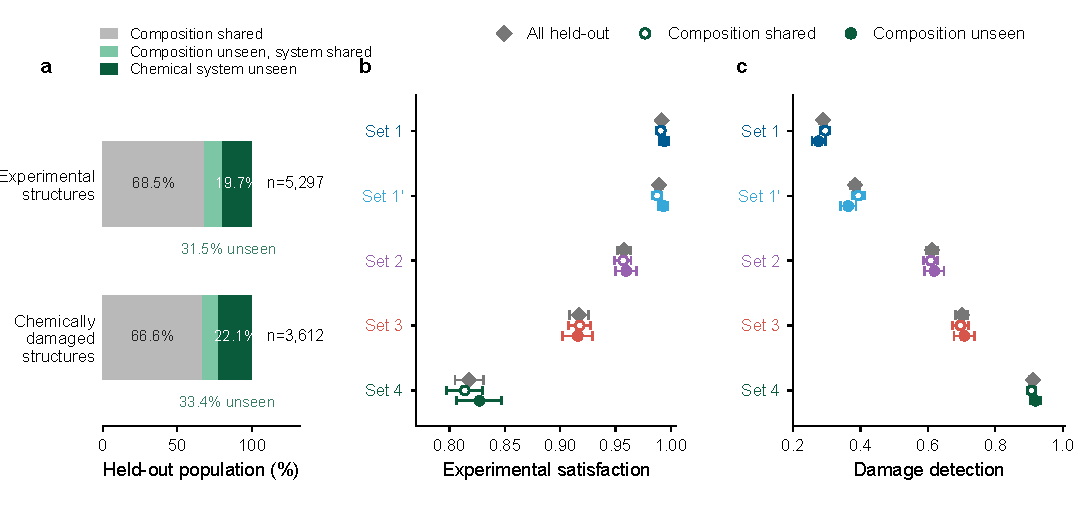
\includegraphics[width=\textwidth]{figs/figS7_pris_composition_holdout.pdf}
  \caption[Frozen PRIS performance on compositions unseen during discovery]{\textbf{Frozen
  PRIS law sets retain their performance on compositions unseen during law discovery.}
  \textbf{a},~Chemistry overlap created by the original structure-identifier split.
  Held-out experimental structures and their chemically damaged counterparts are partitioned
  into compositions present in discovery (grey), unseen compositions whose element set was
  seen (light green), and unseen exact chemical systems (dark green). Damaged structures
  inherit the composition of their experimental parent. \textbf{b},~Experimental-structure
  satisfaction for the five frozen PRIS law sets in the full held-out population (grey
  diamonds), composition-shared subset (open circles) and composition-unseen subset (filled
  circles). \textbf{c},~Damage detection for the same populations. Points are
  structure-weighted estimates; bars are 95\% percentile intervals from 10{,}000 bootstrap
  resamples of whole reduced-composition clusters (seed 20260829). The rules, thresholds and
  missing-feature convention were not changed.}
  \label{sifig:pris-composition-holdout}
\end{figure}
\FloatBarrier

\section{Reproducing the analysis}\label{note:s9}

\begin{verbatim}
# example command-line configurations
# archived five-law set: Law~1 and Law~3--Law~6
python src/apply_rules.py <structure files>
# archived four-law set: Law~1 and Law~3--Law~5
python src/apply_rules.py --set core4 *.cif
# single reduced-distance law, threshold 0.735
python src/apply_rules.py --set single *.cif

# per-law values plus archived exploratory formula
# (not its historical fitted accuracy)
python src/apply_rules.py --verbose --formula a.cif

# figures read paper/data/*.csv
# plotting code does no computation
python src/paper_figs.py

# rebuilding aggregate CSVs first requires the external
# feature store
PRIS_FEATURES=/path/to/features \
  python src/paper_data.py
\end{verbatim}

\textbf{Public benchmark.} Because ICSD is not redistributable and ELEMENTA is
CC-BY-NC-4.0, the benchmark released with this work is built exclusively on the
25,339 COD structures (CC0).

\section{Exact search does not remove omitted-class sensitivity within the tested shallow-tree space}\label{note:s10}

\textbf{Purpose.} To test whether the beam search of \S{}S4 missed a better law set,
we used an exact algorithm that proves optimality within a defined class of trees.

\textbf{Set-up.} The discovery matrix contained 12,632 experimental structures,
8,590 damaged structures, and 79 numerical features available for more than 0.9
of rows. We supplied this matrix to \texttt{pystreed} 1.3.9, which implements
STreeD separable-objective optimal decision trees by dynamic programming. We set
\texttt{continuous\_binarize\_strategy=\allowbreak"quantile"} and
\texttt{n\_thresholds=3}. These settings select candidate splits from each
feature's percentiles. The class of depth-$\leq$3 trees strictly contains the class of conjunctions
explored by beam search. Wall-clock time was 0.8 s at depth 1, 0.7 s at depth 2,
6--28 s at depth 3, and 549 s at depth 4, which was impractical.

\textbf{Moving along the trade-off curve.} Changing the optimisation objective
did \emph{not} move the curve: \texttt{f1-score} and \texttt{accuracy} returned
the same depth-3 tree. The \textbf{cost ratio} did move the curve. It balances
the cost of rejecting an experimental structure against accepting a damaged
structure, and was implemented by sample replication:

{\def\LTcaptype{none} % do not increment counter
\begin{longtable}[]{@{}lll@{}}
\toprule\noalign{}
cost ratio & satisfaction & damage detection \\
\midrule\noalign{}
\endhead
\bottomrule\noalign{}
\endlastfoot
1.00 & 0.8895 & 0.8553 \\
1.50 & 0.9265 & 0.7849 \\
1.75 & 0.9367 & 0.7540 \\
2.00 & 0.9367 & 0.7540 \\
2.25 & 0.9367 & 0.7540 \\
2.50 & 0.9518 & 0.6732 \\
3.00 & 0.9807 & 0.5637 \\
4.00 & 0.9790 & 0.5697 \\
\end{longtable}
}

\textbf{Testing on a damage type omitted during fitting.} We refitted at cost ratio 2.5
with one damage type removed entirely, then tested on that type:

{\def\LTcaptype{none} % do not increment counter
\begin{longtable}[]{@{}p{0.28\linewidth}p{0.31\linewidth}p{0.31\linewidth}@{}}
\toprule\noalign{}
damage type omitted & damage detection on types used in fitting & damage detection on omitted type \\
\midrule\noalign{}
\endhead
\bottomrule\noalign{}
\endlastfoot
D1 uniaxial compression & 0.7553 & 0.2222 \\
D2 cation--cation swap & 0.7048 & 0.1445 \\
D3 random displacement & 0.5310 & 0.6971 \\
D4 isotropic expansion & 0.6903 & 0.0235 \\
D5 cation--anion swap & 0.6747 & 0.0715 \\
\textbf{mean} & \textbf{0.6712} & \textbf{0.2318} \\
\end{longtable}
}

The single-threshold criterion, selected by the same procedure, achieved 0.2819
on seen damage types and 0.2771 on omitted types. For each method, we first took the
absolute seen-versus-omitted detection difference in each of the five leave-one-class-out
fits and then averaged those five differences. The result was 0.506 for the tree and 0.321
for the threshold, a factor of 1.58. For the threshold, the near-zero signed difference
between its seen and omitted means is misleading because class-specific improvements such
as D3 can cancel losses such as D4 and D5 (Supplementary Fig.~\ref{sifig:loko}a).

\textbf{First,} the provably optimal depth-3 tree at satisfaction 0.95 did not
select \rhoc{}. It used \texttt{ecc\_mean}, \texttt{mad\_an\_mean},
\texttt{mad\_range}, \texttt{frac\_like\_bonds}, \texttt{pair\_per\_cat}, and
\texttt{cat\_an\_ratio}.

\textbf{Second,} the direction and magnitude of the change were damage-type specific. This
pattern is consistent with sensitivity to the perturbation procedure, although
it does not isolate the cause.

\textbf{Independent replication.} These numbers were produced twice, by separate agents in
separate environments, from the same stored feature matrix. All values agree to four decimal places.

\textbf{What this result supports.} Within the tested discretized class of depth-$\leq 3$
trees, the in-distribution gain does not survive on average when one damage type is omitted
during fitting. This establishes sensitivity to how damaged structures were generated within
this feature grid. It does not show that the perturbation procedure is the only limitation or
rule out gains from other features, model classes or objectives.

\section{What a one-sided criterion misses, and the condition that repairs it}\label{note:s11}

\textbf{What it misses.} \rhoc{} is a lower bound on the reduced contact ratio, so it cannot detect
a structure that is too open. Damage detection against isotropic expansion
of 20--40\% is 0.002 for \rhoc{} $\geq$ 0.735 and 0.002 for \rhoc{} $\geq$ 0.804.
The complete threshold sweep shows this expansion blind spot across the tested range
(Supplementary Fig.~\ref{sifig:threshold}).

\textbf{An unconditional upper bound adds no value when required satisfaction is at least about 95\%.}
We scanned $\tau$\_lo $\in$ {[}0.60, 1.00{]} $\times$ $\tau$\_hi $\in$
{[}1.00, 3.60{]}. One-sided and two-sided criteria were compared at the same
required satisfaction:

{\def\LTcaptype{none} % do not increment counter
\begin{longtable}[]{@{}llll@{}}
\toprule\noalign{}
minimum satisfaction & best one-sided & best two-sided & gain \\
\midrule\noalign{}
\endhead
\bottomrule\noalign{}
\endlastfoot
0.99 & \rhoc{} $\geq$ 0.735, 0.2881 & {[}0.73, 3.04{]}, 0.2823 & $-$0.006 \\
0.98 & \rhoc{} $\geq$ 0.780, 0.3674 & {[}0.78, 3.26{]}, 0.3682 & +0.001 \\
0.97 & \rhoc{} $\geq$ 0.800, 0.4064 & {[}0.80, 2.80{]}, 0.4097 & +0.003 \\
0.96 & \rhoc{} $\geq$ 0.815, 0.4377 & {[}0.81, 2.40{]}, 0.4343 & $-$0.003 \\
0.95 & \rhoc{} $\geq$ 0.830, 0.4690 & {[}0.83, 3.58{]}, 0.4695 & +0.000 \\
0.94 & \rhoc{} $\geq$ 0.835, 0.4785 & \textbf{{[}0.75, 1.12{]}, 0.5126} & \textbf{+0.034} \\
0.92 & \rhoc{} $\geq$ 0.850, 0.5073 & \textbf{{[}0.80, 1.08{]}, 0.6179} & \textbf{+0.111} \\
0.90 & \rhoc{} $\geq$ 0.860, 0.5227 & \textbf{{[}0.83, 1.08{]}, 0.6806} & \textbf{+0.158} \\
\end{longtable}
}

The optimal upper bound changes abruptly with the allowed loss in satisfaction.
It is effectively infinite above 0.95 and snaps to $\approx$1.08 below it. Our
initial report included only the 0.99 row, producing the false conclusion logged
as R11 (Supplementary Fig.~\ref{sifig:band-grid}).

\textbf{Chemical character of the upper tail.} The 626 experimental structures
with \rhoc{} \textgreater{} 1.08 (4.97\% of 12,601) lie outside the ionic domain:

{\def\LTcaptype{none} % do not increment counter
\begin{longtable}[]{@{}lll@{}}
\toprule\noalign{}
quantity & median, \rhoc{} $\leq$ 1.08 & median, \rhoc{} \textgreater{} 1.08 \\
\midrule\noalign{}
\endhead
\bottomrule\noalign{}
\endlastfoot
Pauling ionicity \emph{f}\_i & 0.508 & 0.111 \\
electronegativity difference $\Delta$$\chi$ & 1.683 & 0.688 \\
global instability index & 0.211 & 1.171 \\
MEFIR mismatch (max) & 0.008 & 1.956 \\
Pauling rule 2 satisfied (frac. of sites) & 0.833 & 0.000 \\
Shannon packing fraction & 0.659 & 0.093 \\
\end{longtable}
}

The Shannon ionic-radius model does not apply to these structures, even though
they satisfy the charge-balance filter. Charge balance alone therefore does not
establish applicability of the ionic-radius model. Supplementary
Fig.~\ref{sifig:chemistry} resolves the response by anion chemistry and shows
where the ionicity condition adds damage detection.

\textbf{The conditional law.} Above \rhoc{} = 1.05 lie 0.62\% of ionic experimental structures (\emph{f}\_i \textgreater{} 0.5),
10.07\% of non-ionic experimental structures, and 96.14\% of expanded
structures. These distributions motivate the following conditional law:

\begin{quote}
\textbf{Set~1$'$} \rhoc{} $\geq$ 0.735 \textbf{and} ( \emph{f}\_i $\leq$ 0.50 \textbf{or} \rhoc{} $\leq$ 1.05 )
\end{quote}

{\footnotesize
\def\LTcaptype{none} % do not increment counter
\begin{longtable}[]{@{}
  >{\raggedright\arraybackslash}p{(\linewidth - 14\tabcolsep) * \real{0.1250}}
  >{\raggedright\arraybackslash}p{(\linewidth - 14\tabcolsep) * \real{0.1250}}
  >{\raggedright\arraybackslash}p{(\linewidth - 14\tabcolsep) * \real{0.1250}}
  >{\raggedright\arraybackslash}p{(\linewidth - 14\tabcolsep) * \real{0.1250}}
  >{\raggedright\arraybackslash}p{(\linewidth - 14\tabcolsep) * \real{0.1250}}
  >{\raggedright\arraybackslash}p{(\linewidth - 14\tabcolsep) * \real{0.1250}}
  >{\raggedright\arraybackslash}p{(\linewidth - 14\tabcolsep) * \real{0.1250}}
  >{\raggedright\arraybackslash}p{(\linewidth - 14\tabcolsep) * \real{0.1250}}@{}}
\toprule\noalign{}
\begin{minipage}[b]{\linewidth}\raggedright
\end{minipage} & \begin{minipage}[b]{\linewidth}\raggedright
satisfaction
\end{minipage} & \begin{minipage}[b]{\linewidth}\raggedright
damage detection
\end{minipage} & \begin{minipage}[b]{\linewidth}\raggedright
D1
\end{minipage} & \begin{minipage}[b]{\linewidth}\raggedright
D2
\end{minipage} & \begin{minipage}[b]{\linewidth}\raggedright
D3
\end{minipage} & \begin{minipage}[b]{\linewidth}\raggedright
D4
\end{minipage} & \begin{minipage}[b]{\linewidth}\raggedright
D5
\end{minipage} \\
\midrule\noalign{}
\endhead
\bottomrule\noalign{}
\endlastfoot
Set~1 (one-sided) & 0.9900 & 0.2881 & 0.192 & 0.324 & 0.879 & 0.002 & 0.019 \\
two-sided, unconditional & 0.9900 & 0.2823 & 0.173 & 0.307 & 0.875 & 0.011 & 0.018 \\
\textbf{Set~1$'$ (conditional)} & \textbf{0.9870} & \textbf{0.3879} & 0.193 & 0.324 & 0.880 & \textbf{0.513} & 0.023 \\
\end{longtable}
}

The full law-set sequence progressively closes the expansion blind spot
(Supplementary Fig.~\ref{sifig:unguarded}).

\textbf{Testing Set~1$'$ on a damage type omitted during fitting.} The condition
and threshold were selected using only the four retained classes, then applied
to the omitted class:

{\def\LTcaptype{none} % do not increment counter
\begin{longtable}[]{@{}
  >{\raggedright\arraybackslash}p{(\linewidth - 8\tabcolsep) * \real{0.2000}}
  >{\raggedright\arraybackslash}p{(\linewidth - 8\tabcolsep) * \real{0.2000}}
  >{\raggedright\arraybackslash}p{(\linewidth - 8\tabcolsep) * \real{0.2000}}
  >{\raggedright\arraybackslash}p{(\linewidth - 8\tabcolsep) * \real{0.2000}}
  >{\raggedright\arraybackslash}p{(\linewidth - 8\tabcolsep) * \real{0.2000}}@{}}
\toprule\noalign{}
\begin{minipage}[b]{\linewidth}\raggedright
damage type omitted
\end{minipage} & \begin{minipage}[b]{\linewidth}\raggedright
threshold selected
\end{minipage} & \begin{minipage}[b]{\linewidth}\raggedright
damage detection, omitted type
\end{minipage} & \begin{minipage}[b]{\linewidth}\raggedright
one-sided baseline
\end{minipage} & \begin{minipage}[b]{\linewidth}\raggedright
gain
\end{minipage} \\
\midrule\noalign{}
\endhead
\bottomrule\noalign{}
\endlastfoot
D1 & 1.05 & 0.1954 & 0.1949 & +0.0005 \\
D2 & 1.05 & 0.3243 & 0.3235 & +0.0008 \\
D3 & 1.05 & 0.8798 & 0.8793 & +0.0005 \\
\textbf{D4} & \textbf{1.05} & \textbf{0.5127} & \textbf{0.0024} & \textbf{+0.5102} \\
D5 & 1.05 & 0.0226 & 0.0189 & +0.0037 \\
\end{longtable}
}

The same threshold was selected in all five repeats. Its performance on each
omitted type isolates the contribution of the conditional upper-contact law
(Supplementary Fig.~\ref{sifig:loko}b).

\textbf{Stated limitation.} Omitting one damage type during fitting tests whether the selected threshold
works on that type. This leave-one-type test does not establish whether the mathematical form would have
been discovered without prior knowledge of that type of damage. We tested a two-sided
band because the controlled-damage benchmark included isotropically expanded structures.
A different damage type may require reconsidering the form, not only the threshold.

\begin{figure}[!htbp]
  \centering
  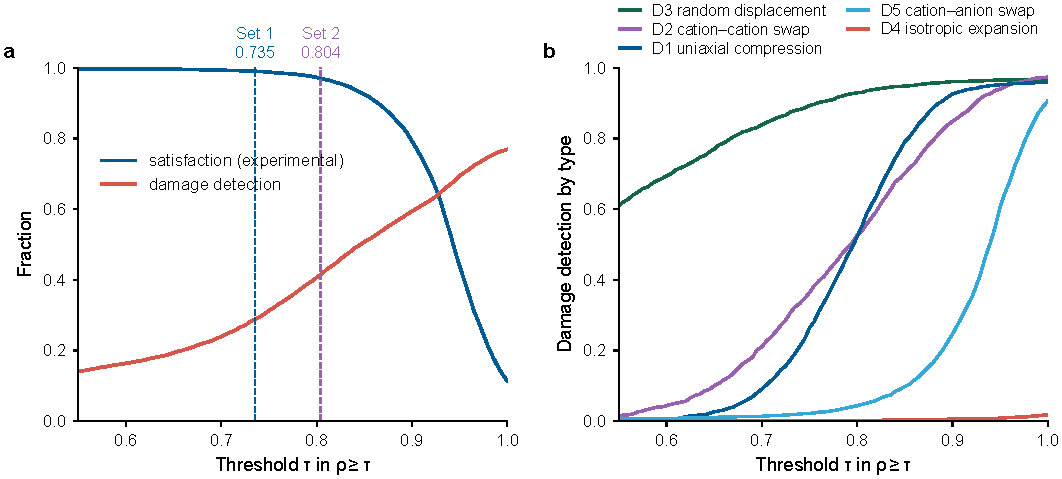
\includegraphics[width=\textwidth]{figs/figS8_threshold.pdf}
  \caption[Contact-threshold sensitivity]{\textbf{Sensitivity to the Law~1 contact
  threshold.} \textbf{a},~Experimental-structure satisfaction and pooled damage
  detection across a discovery-split sweep of the lower-contact threshold \(\tau\)
  in \(\rhoc{}\geq\tau\). Dashed vertical lines identify thresholds used by the
  labelled PRIS law sets. \textbf{b},~The same sweep resolved by the five
  composition-preserving perturbation classes. Colour identifies the class.}
  \label{sifig:threshold}
\end{figure}

\begin{figure}[!htbp]
  \centering
  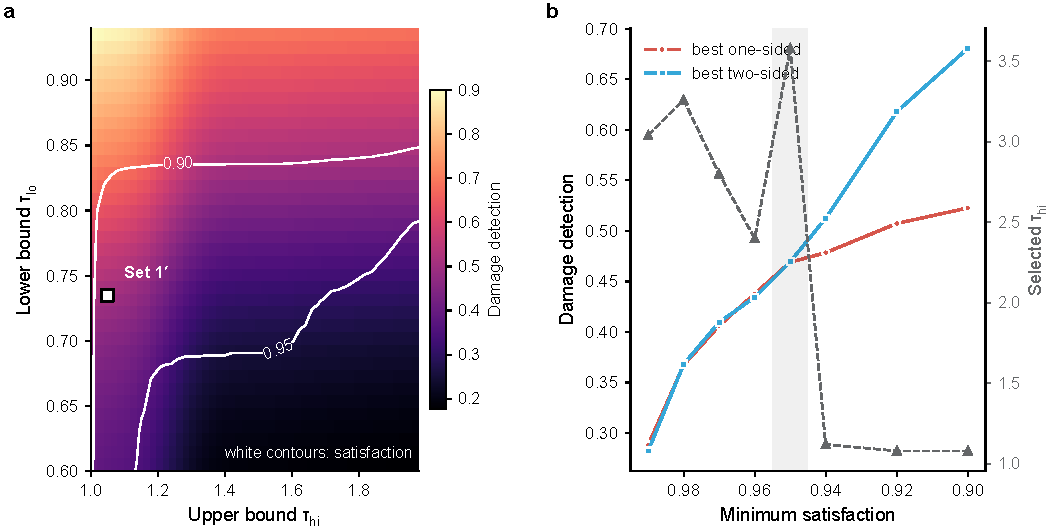
\includegraphics[width=\textwidth]{figs/figS9_band_grid.pdf}
  \caption[Two-dimensional contact-band scan]{\textbf{Two-dimensional scan of
  contact-band bounds.} \textbf{a},~On the discovery split, lower and upper
  reduced-contact bounds define the axes. Colour maps pooled damage detection.
  White contours mark experimental-structure satisfaction, and the square marks
  Set~1$'$. \textbf{b},~Minimum satisfaction is plotted against the
  best one-sided and two-sided detection rates. Grey triangles on the right axis
  give the selected upper bound.}
  \label{sifig:band-grid}
\end{figure}

\begin{figure}[!htbp]
  \centering
  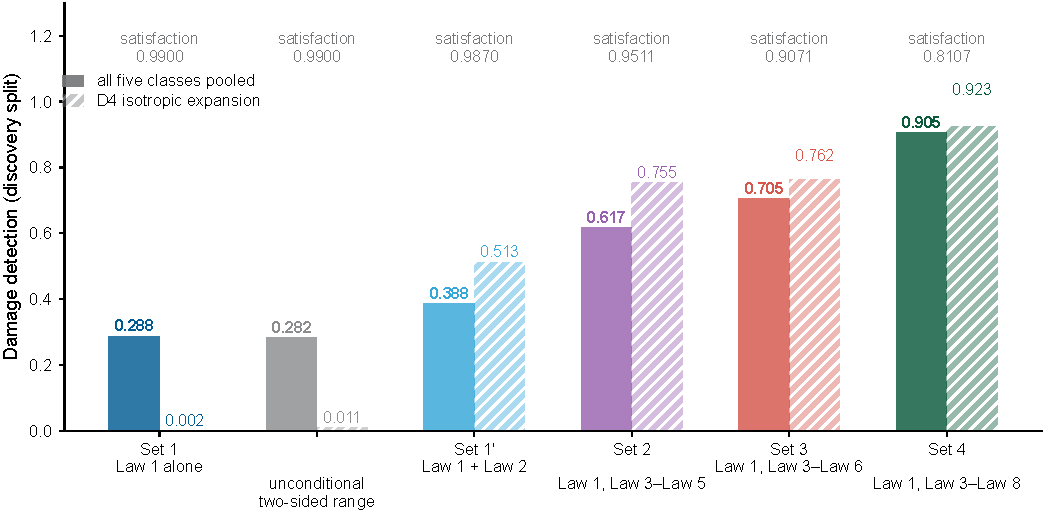
\includegraphics[width=\textwidth]{figs/figS10_unguarded_band.pdf}
  \caption[Law sets and an unconditional two-sided band]{\textbf{PRIS law sets and
  an unconditional two-sided contact band.} Discovery-split criteria are arranged
  from Law~1 through the successive PRIS law sets. The unconditional two-sided
  range is included as a comparator. Solid bars show pooled detection across
  perturbation classes, whereas hatched bars isolate isotropic expansion. Colours
  identify the criteria. Text above each group gives experimental-structure
  satisfaction.}
  \label{sifig:unguarded}
\end{figure}

\begin{figure}[!htbp]
  \centering
  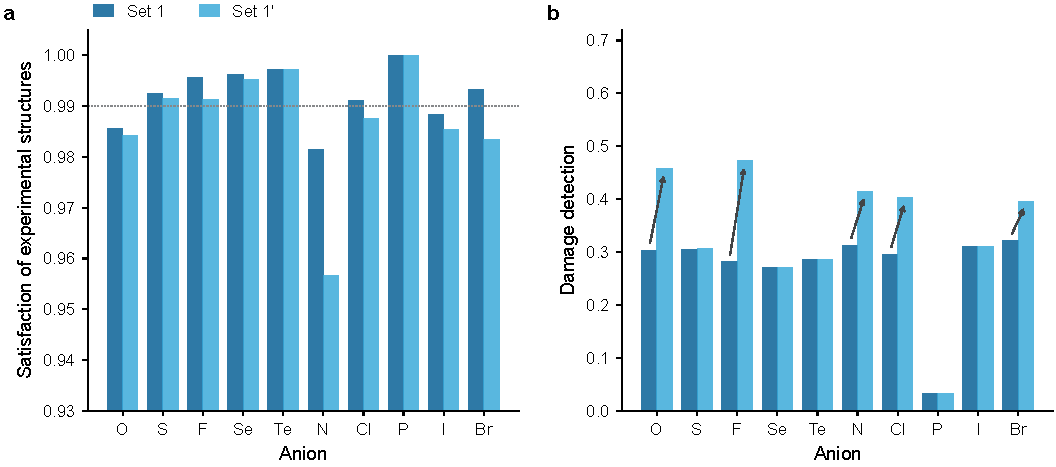
\includegraphics[width=\textwidth]{figs/figS11_chemistry.pdf}
  \caption[Performance by anion family]{\textbf{Contact-law performance by dominant
  anion family.} Discovery-split structures are grouped by dominant anion along
  both horizontal axes. \textbf{a},~Paired bars compare experimental-structure
  satisfaction for Set~1 and conditional Set~1$'$. The dotted line marks the
  reference level. \textbf{b},~Paired bars show pooled damage detection for the
  same criteria and families. Arrows mark differences selected by the display
  rule; they do not denote statistical tests.}
  \label{sifig:chemistry}
\end{figure}

\begin{figure}[!htbp]
  \centering
  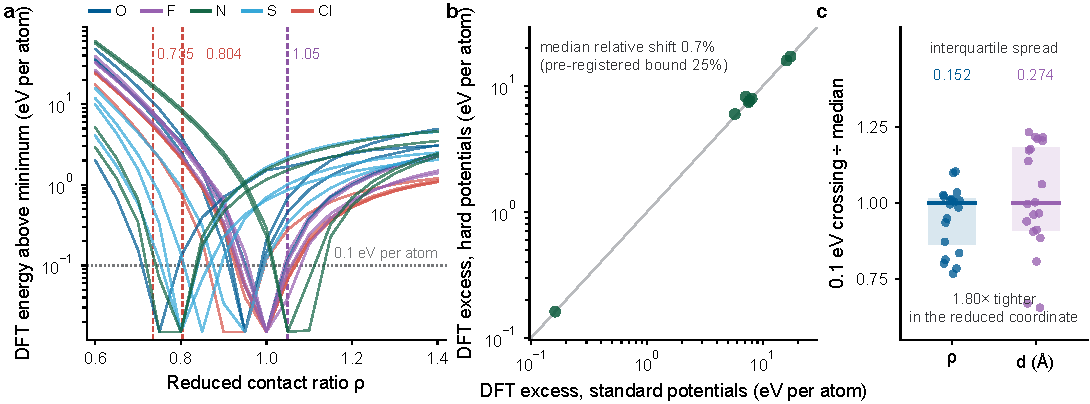
\includegraphics[width=\textwidth]{figs/figS12_dft_e1_landscape.pdf}
  \caption[First-principles energy landscape behind the contact thresholds]{\textbf{The contact thresholds measured from first principles.} \textbf{a},~Each line is one of
  twenty experimental compounds rigidly scaled along the reduced-contact
  coordinate and evaluated with plane-wave DFT. The vertical axis is the DFT
  energy above each compound's own minimum, and colour gives the dominant anion.
  The dotted horizontal line marks 0.1\,eV per atom, the pre-registered cost of a
  chemical rather than geometric short contact. Dashed vertical lines mark the
  Law~1 floors of 0.735 and 0.804 and the Law~2 ceiling of 1.05. Every chemistry
  rises steeply below the floors, so the thresholds do not average soft and stiff
  cases. \textbf{b},~Eight compounds were recomputed with hard potentials, which
  freeze smaller cores, and compared with the standard set. Both axes report DFT
  energy excess at the floor, and the diagonal marks equality. The annotation
  gives the median relative shift against the
  threshold fixed before calculation.
  \textbf{c},~Each point is the contact at which a compound first pays the
  pre-registered cost. Reduced-contact and \AA{} crossings are each normalised by
  their own median. Boxes span the interquartile range, and the number above each
  box gives its width. The crossing is 1.80 times more tightly localised in the
  reduced coordinate, enabling comparison across chemistries.}
  \label{sifig:dft-e1-landscape}
\end{figure}

\begin{figure}[!htbp]
  \centering
  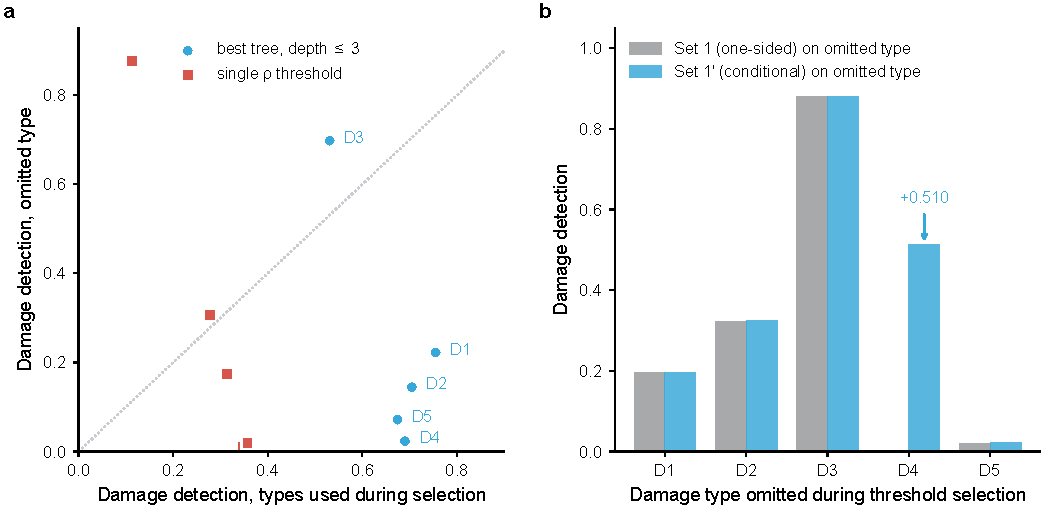
\includegraphics[width=\textwidth]{figs/figS13_loko.pdf}
  \caption[Leave-one-perturbation-out tests]{\textbf{Leave-one-perturbation-out
  evaluation of selected contact criteria.} \textbf{a},~Each point represents one
  perturbation class omitted during selection. The axes give damage detection on the
  retained classes and on the omitted class. Blue circles denote the depth-limited
  tree, red squares denote the single \rhoc{} threshold, and the dotted diagonal marks
  equality. \textbf{b},~Paired bars compare one-sided Set~1 and conditional Set~1$'$ on each
  omitted class.}
  \label{sifig:loko}
\end{figure}

\begin{figure}[!htbp]
  \centering
  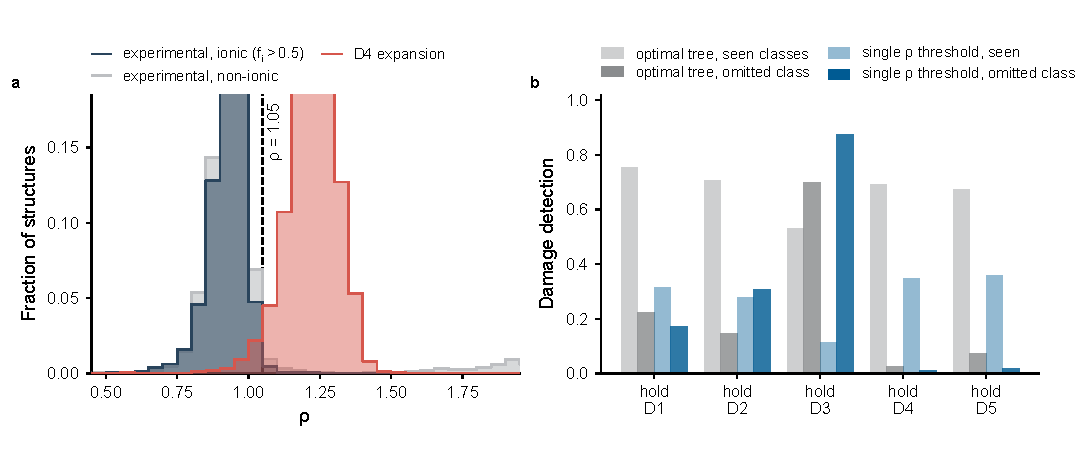
\includegraphics[width=\textwidth]{figs/figS14_validation_boundary_omission.pdf}
  \caption[Conditional contact thresholds and leave-one-damage-class-out evaluation]{\textbf{Conditional contact thresholds and leave-one-damage-class-out evaluation.}
  \textbf{a},~Normalised reduced-contact distributions for experimental structures
  separated by ionicity and for isotropically expanded structures. Filled step curves
  identify the cohorts, and the vertical dashed line marks the conditional upper bound.
  \textbf{b},~Damage detection for a depth-limited tree and a single \rhoc{} threshold
  when each perturbation class is omitted in turn. Grey and blue identify the two model
  classes, while pale and solid bars distinguish retained and omitted perturbation
  classes.}
  \label{sifig:validation-boundary-omission}
\end{figure}

\section{Exact perturbation operators used in D1--D5}\label{note:s12}

The exact procedures are reproduced below:

{\def\LTcaptype{none} % do not increment counter
\begin{longtable}[]{@{}
  >{\raggedright\arraybackslash}p{(\linewidth - 2\tabcolsep) * \real{0.5000}}
  >{\raggedright\arraybackslash}p{(\linewidth - 2\tabcolsep) * \real{0.5000}}@{}}
\toprule\noalign{}
\begin{minipage}[b]{\linewidth}\raggedright
class
\end{minipage} & \begin{minipage}[b]{\linewidth}\raggedright
operation
\end{minipage} \\
\midrule\noalign{}
\endhead
\bottomrule\noalign{}
\endlastfoot
\textbf{D1} & anisotropic compression: one randomly chosen lattice axis scaled by 1 $-$ \emph{u}, \emph{u} \textasciitilde{} U(0.15, 0.30) \\
\textbf{D2} & cation--cation swap between two cations whose \textbf{formal charges differ by $\geq$ 1}, with the charges swapped alongside the species \\
\textbf{D3} & random displacement of every site, Gaussian, amplitude \emph{u} \textasciitilde{} U(0.3, 0.8) \AA{} \\
\textbf{D4} & isotropic expansion: all lattice vectors scaled by 1 + \emph{u}, \emph{u} \textasciitilde{} U(0.20, 0.40) \\
\textbf{D5} & cation--anion swap: composition and stoichiometry unchanged, charge arrangement destroyed \\
\end{longtable}
}

The charge-difference requirement in D2 was the subject of refutation R1. The
original implementation swapped species without swapping charges. Consequently,
the Madelung energy change was exactly zero for 100\% of samples. The resulting
``structure'' was only a relabelling of the original.

\section{Composition-grouped ranking separates decision rate from accuracy}\label{note:s13}

Within each composition, we paired every experimentally recorded Materials
Project entry with every entry lacking an experimental record. We restricted the
analysis to charge-balanced ionic compositions. The resulting cohort contained
1{,}508 compositions, 6{,}758 structures, and 18{,}920 pairs.

A criterion provides a usable pairwise comparison when its two values differ
beyond numerical tolerance. A tie provides no comparison. The pair-level decision
rate in Supplementary Fig.~\ref{sifig:polymorph-ranking}a is one minus the
fraction of tied pairs. It is distinct from the group-level tie rate in panel b.
Accuracy is calculated only for usable pairs; ties count as neither successes nor
errors. The Top-1 hit rate is the expected fraction of experimentally recorded
entries among structures tied for the criterion's minimum. Its random baseline
is the experimentally recorded fraction in that group. The archived ranking
table reports Top-1 lift alongside decision rate. Set~4 distinguished 28.2\% of
all pairs and selected no unique structure in 85.1\% of composition groups.

Every statistic is first calculated within a composition. We then average with
equal weight across compositions for which that criterion yields a usable
comparison. The number of contributing groups therefore differs among criteria,
and their accuracies do not share one set of pairs. Explicit tie handling and
group-equal weighting are both essential.

In R10, counting 77.7\% of ties as errors produced the false claim that
Pauling's rules perform worse than chance. In R9, pair weighting allowed
SiO$_2$, which supplies 43.6\% of all pairs, to dominate the comparison. Under
pair weighting, density versus formation-energy accuracy was 0.7103 versus
0.6476. Group-equal weighting reversed it to 0.6347 versus 0.7451.

Confidence intervals come from a cluster bootstrap that resamples composition
groups with replacement and recomputes the group-equal statistic. This unit
preserves within-composition correlation. Pair-level resampling would narrow the
intervals to a meaningless width. Folds are split by composition group. The
bootstrap used $B=500$ replicates and seed 20260728.

\section{Supplementary figure conventions and source data}\label{note:s14}

All supplementary figures are drawn in Arial and carry no in-panel titles. The subject of
each figure is stated in the first clause of its caption. Source data accompany the paper, and the plotting code performs no computation.

\section{PRIS-derived synthesis score for composition-held-out ranking}\label{note:s15}

This note documents the score reported in the main text as the PRIS-derived synthesis score
(PSS).

\textbf{Why a new analysis.} The plausibility laws were fitted to damage detection,
whereas synthesizability screening benefits from a continuous ordering of structures
within the same composition. PSS was therefore fitted directly to the
experimental-record label under the composition-held-out protocol documented here.

\textbf{Connection to the wider programme.} This analysis and the refit in Section
S16 belong to the autonomous programme documented in Section S1. Both were executed
in sessions dated 2026-08-14, after the first authorised reserve evaluation.
They reuse the programme's data, feature conventions, and evaluation code. The
unified statistics in Section S1 include both analyses.

\textbf{Pre-registration.} The synthesis-score plan was fixed before fitting, and
its SHA-256 was recorded in the repository. Revision 1 added a minimum decision
rate of $\geq0.99$ after development search found a high-accuracy solution that
ranked too few pairs. Revision 2 added a secondary hybrid model with its form
fixed before evaluation. Both revisions predated the single held-out evaluation.
Before computing any new row, we reproduced four published baselines to four
decimal places: Pauling 5, \rhoc{}, volume per atom, and DFT
$E_{\mathrm{hull}}$.

\textbf{Split.} A seeded hash of each composition string assigned all 1{,}508
two-class groups to development or held-out sets. Development contained 919
groups, 4{,}187 structures, and 14{,}563 pairs. Held-out evaluation contained 589
groups, 2{,}571 structures, and 4{,}357 pairs. SiO$_2$, which supplies 0.436 of
all pairs, fell in the development set. The held-out results are therefore free
of the known single-composition dominance in R9. The evaluation script accessed
the held-out set exactly once, after every coefficient was fixed and hashed.

\textbf{Feature pool.} We began with 85 stored structural features in the task
table. The pre-registered exclusion list removed extensive counts, Ewald totals,
and a table-availability artefact. Nine features were then added by physical
function. Symmetry features comprised space-group number, crystal-system rank,
and distinct-site fraction at two tolerances. Classical-repulsion features were
$\sum (r_{\mathrm{sum}}/d)^9/N$ and
$\sum \exp[(r_{\mathrm{sum}}-d)/0.345\,\text{\AA}]/N$, resolved by charge-sign
pair. The remaining additions were cation--anion elastic strain and mass density.
No feature uses DFT output. Charges are composition-only integer valences, and
radii are Shannon radii, as throughout this work.

\textbf{Model class.} We used an antisymmetric pairwise logistic score with no
intercept. Reversing a pair therefore reverses the score without changing its
magnitude. Features were standardised using development data, and missing values
were handled by the frozen preprocessing statistics. Pairs received equal weight
within each composition. Greedy forward selection used five-fold grouped
cross-validation, at most eight terms, and a minimum gain of $0.002$. The final
model was refitted on all development data. Its coefficients and preprocessing
statistics were stored in a SHA-256-hashed JSON file before held-out evaluation.

\textbf{Development result.} Forward selection added terms in this order:
(1) $\overline{E_{\mathrm{M}}/|z|}$, score 0.6299; (2) distinct-site fraction,
0.6870; (3) mean relative bond-valence deviation, 0.7214; (4) volume per atom,
0.7344; (5) maximum polyhedral connectivity, 0.7442; and (6) fraction of
isolated polyhedra, 0.7548. A seventh candidate gained $+0.0017$, below the
pre-registered minimum, and was not retained.

An L2-regularised model using all allowed features scored 0.7572. DFT hull
energy scored 0.7500 on the same development groups. The archive contains the
fixed coefficients, preprocessing statistics, SHA-256 hashes, and complete
single-feature audit. Leading single features were distinct-site fraction
(0.6837 at decision rate 0.79), the bond-valence family (0.664--0.667 at decision
rate $\geq0.99$), and density (0.6495).

\textbf{Experimental records.} The synthesis task uses the same classification of
experimentally recorded structures and structures without an experimental record as Section S13.

\textbf{On held-out data.} Across 589 held-out groups, PSS scored 0.6811 at
decision rate 1.000. The full-feature-pool variant scored 0.7059. The hybrid with
hull energy, whose form was fixed before evaluation, scored 0.6865. Reference
scores were 0.7503 for DFT hull energy, 0.6346 for volume per atom, 0.6219 for
Shannon packing, and 0.5597 for \rhoc{}. Paired cluster-bootstrap differences
were $-0.0646$ $[-0.1043,-0.0267]$ for PSS minus hull and $-0.0592$
$[-0.0963,-0.0234]$ for hybrid minus hull.

PSS decided every group and outperformed every single structural score. Its
Top-1 lift was $+0.2003$, compared with $+0.2971$ for hull energy. Neither PSS
nor the hybrid overtook hull energy overall. As specified before evaluation, the
main text reports that PSS does not match DFT accuracy and gives the difference
with its interval. The decline from 0.7548 in grouped cross-validation to 0.6811
on held-out compositions measures optimism from repeated development. The log
records exactly one held-out evaluation.

\textbf{Accuracy among confident comparisons.} This analysis was performed after
held-out evaluation. For each criterion, pairs were ordered by $|\Delta s|$, the
absolute pairwise score difference. The table reports pair-level accuracy and
cluster confidence intervals; the complete resolution table is archived.

{\def\LTcaptype{none}
\begin{longtable}[]{@{}lllll@{}}
\toprule\noalign{}
pairs kept & PSS & 95\% CI & $E_{\mathrm{hull}}$ & paired $\Delta$ [CI] \\
\midrule\noalign{}
\endhead
\bottomrule\noalign{}
\endlastfoot
1.00 & 0.7384 & [0.708, 0.777] & 0.8074 & --- \\
0.50 & 0.8237 & [0.785, 0.851] & 0.8476 & $-0.024$ $[-0.082, +0.062]$ \\
0.30 & 0.9135 & [0.863, 0.944] & 0.8187 & $+0.095$ $[-0.005, +0.139]$ \\
0.20 & 0.9437 & [0.896, 0.969] & 0.8439 & $+0.100$ $[+0.012, +0.199]$ \\
0.10 & 0.9655 & [0.905, 0.988] & 0.9241 & $+0.041$ $[+0.000, +0.217]$ \\
\end{longtable}
}

The retained-pair fractions were examined after the single held-out evaluation;
this breakdown is descriptive rather than pre-registered. At the most confident
fifth, CeSe$_2$ supplies 0.245 of pairs. The all-pair values differ from the
reported group-equal comparison of 0.6811 versus 0.7503 because held-out groups
still differ in size, even without silica.

Only the most confident fifth has a paired interval excluding zero. A
Bonferroni-adjusted 99 per cent interval across the five examined fractions still
excludes zero ($+0.100$ $[+0.004,+0.220]$). Removing the most represented
composition strengthens the difference to $+0.159$ $[+0.033,+0.213]$. At
retained fractions of 100\%, 50\%, 30\%, 20\%, and 10\%, the largest-composition
shares are 0.331, 0.120, 0.174, 0.245, and 0.450, respectively. This remains an
exploratory breakdown of one held-out evaluation.

\textbf{Stability of the coefficients and correlation of the terms.} The six
terms remained fixed; only their coefficients were re-estimated. The feature
search was not reopened. Every result below uses only the 919 development groups,
comprising 4{,}187 structures and 14{,}563 within-composition pairs, under frozen
preprocessing statistics. The held-out groups were not evaluated again.

Refitting random subsets of development structures moved individual coefficients
but barely changed the score ranking. Across 200 draws at each size, mean
Spearman agreement with the published score was 0.973 on half the structures and
0.998 on nine tenths. Mean cosine similarity of the coefficient vectors was
0.983 and 0.998, respectively.

Coefficient magnitudes were less stable and varied by term. On half the
structures, the 95\% range spanned $\pm21\%$ of the published
\(\widetilde\eta_{\mathrm{site}}\) coefficient but $\pm116\%$ of
\(\widetilde M_z\). Every coefficient retained its published sign in at least
95.5\% of draws (Supplementary Fig.~\ref{sifig:pss-coefficient-stability}a,c).

A cluster bootstrap over composition groups used all development data and the
interval convention of Section~S13. It produced the same term ordering:
\(|\beta|/\mathrm{SE}\) ranged from 12.1 for
\(\widetilde\eta_{\mathrm{site}}\) to 2.0 for \(\widetilde M_z\). Every
coefficient retained its sign in at least 99.5\% of resamples (Supplementary
Fig.~\ref{sifig:pss-coefficient-stability}b). The development data fix the signs
and relative weights; an individual coefficient should not be read to its second
decimal.

\begin{figure}[!htbp]
  \centering
  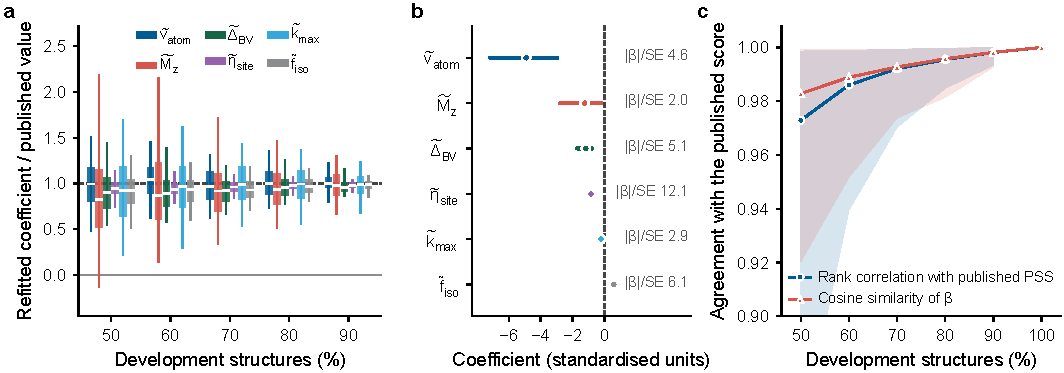
\includegraphics[width=\textwidth]{figs/figS15_pss_coefficient_stability.pdf}
  \caption[Coefficient stability of the fitted synthesis score]{\textbf{Coefficient stability
  of the fitted synthesis score under resampling of the development set.} The six terms are
  held fixed and only their coefficients are re-estimated.
  \textbf{a},~Refitted coefficients divided by their published values for 200
  random subsets at each size. Boxes span the interquartile range, white bars mark
  medians, and whiskers span the 2.5th to 97.5th percentiles. The dashed line
  marks the published value. \textbf{b},~Cluster-bootstrap coefficient intervals
  over all development composition groups ($B=2{,}000$). Intervals span the 2.5th
  to 97.5th percentiles. Circles mark published values, and right-hand labels give
  each coefficient divided by its bootstrap standard error. \textbf{c},~Agreement
  between each refitted score and the published score. The two metrics are
  Spearman rank correlation across development structures and cosine similarity
  between coefficient vectors. Lines give means; shading spans the 2.5th to
  97.5th percentiles.}
  \label{sifig:pss-coefficient-stability}
\end{figure}

The six terms are correlated without being redundant. Across structures, the
strongest Spearman correlations are $-0.51$ between \(\widetilde k_{\max}\) and
\(\widetilde f_{\mathrm{iso}}\), and 0.50 between
\(\widetilde v_{\mathrm{atom}}\) and \(\widetilde M_z\). The pairwise fit instead
uses within-composition differences. In that space, every correlation is below
$|0.36|$, every variance inflation factor is at most 1.29, and the design
correlation matrix has condition number 3.58 (Supplementary
Fig.~\ref{sifig:pss-term-correlation}). The coefficient spread in Supplementary
Fig.~\ref{sifig:pss-coefficient-stability}a therefore reflects the number of
independent composition groups, not near-duplication among terms.

\begin{figure}[!htbp]
  \centering
  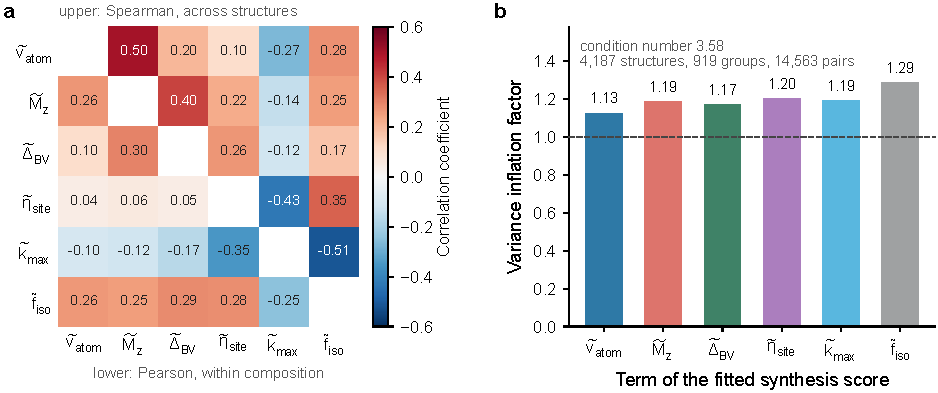
\includegraphics[width=\textwidth]{figs/figS16_pss_term_correlation.pdf}
  \caption[Correlation among the terms of the fitted synthesis score]{\textbf{Correlation
  among the six terms of the fitted synthesis score.}
  \textbf{a},~Correlation matrix of the standardised terms on the development set. Entries
  above the diagonal are Spearman correlations across structures; entries below it are Pearson
  correlations of the within-composition differences that the pairwise fit uses.
  \textbf{b},~Variance inflation factors of the same within-composition design, with the dashed
  line marking the uncorrelated value of one. The condition number of the design correlation
  matrix is given in the panel.}
  \label{sifig:pss-term-correlation}
\end{figure}

\section{PRIS and PSS track predicted synthesizability across two PU models}\label{note:pu-transfer}

\textbf{Positive--unlabelled (PU) learning lineage and expanded pool.} Jang et
al. introduced bagged PU-CGCNN and the crystal-likeness score (CLscore). Their
training data comprised 46{,}781 ICSD-linked Materials Project positives and
77{,}734 virtual unlabelled structures \cite{jang2020structure}. A later study
applied the pretrained CLscore model to 1{,}401{,}562 theoretical structures. It
selected 80{,}000 low-CLscore candidates for a crystal-synthesizability language
model \cite{song2025llm}.

Here, we expanded the positive set to 99{,}162 structures: 73{,}823 from ICSD
and 25{,}339 from COD. We expanded the unlabelled pool to 8{,}125{,}976 LeMat
and ELEMENTA candidates \cite{ramlaoui2025lemat,elementa2025dataset}.

We retrained a 50-bag CGCNN-PU model and fitted 50 MLP PU heads to frozen
128-dimensional MatterSim-v1.0.0-1M representations \cite{yang2024mattersim}.
The two models agreed on 364{,}771 low-CLscore records. Exact-CIF deduplication
removed 179 repeats, leaving 364{,}592 unique PU-selected hard-negative
structures for analysis.

\textbf{Full-pool comparison.} Set~1--Set~4 were applied as independent law-set
choices. Set~1 gave 94.8\% experimental-structure satisfaction and 0.2\%
hard-negative screening. The corresponding values were 88.3\% and 1.8\% for
Set~2, 87.1\% and 1.9\% for Set~3, and 80.7\% and 51.9\% for Set~4. PSS was
evaluated as a continuous threshold curve. At 80.7\% experimental-structure
satisfaction, it screened 83.7\% of the hard-negative pool.

All six PSS descriptors were observed for 21{,}477 experimental structures and
135 hard negatives. For all other records, unavailable descriptors were replaced
with medians fixed on the PSS training data before this analysis.

\textbf{Mechanism attribution.} Fractional attribution preserves the logical OR
that defines Set~4. A structure violating \(k\) laws contributes \(1/k\) to each
violated law, so the shares sum to the complete violation rate. A complementary
leave-one-law-out calculation removes one law and recomputes both
experimental-structure satisfaction and hard-negative screening.

Law~7 supplies 50.28 percentage points of the 51.9\% hard-negative screening
rate. Removing it loses 49.49 percentage points of screening while recovering
5.00 percentage points of experimental-structure satisfaction. Law~1 contributes
more strongly to the controlled-damage benchmark. Different mechanisms therefore
dominate the two tasks (Supplementary Fig.~\ref{sifig:l4-contribution}a,b).

\begin{figure}[!htbp]
  \centering
  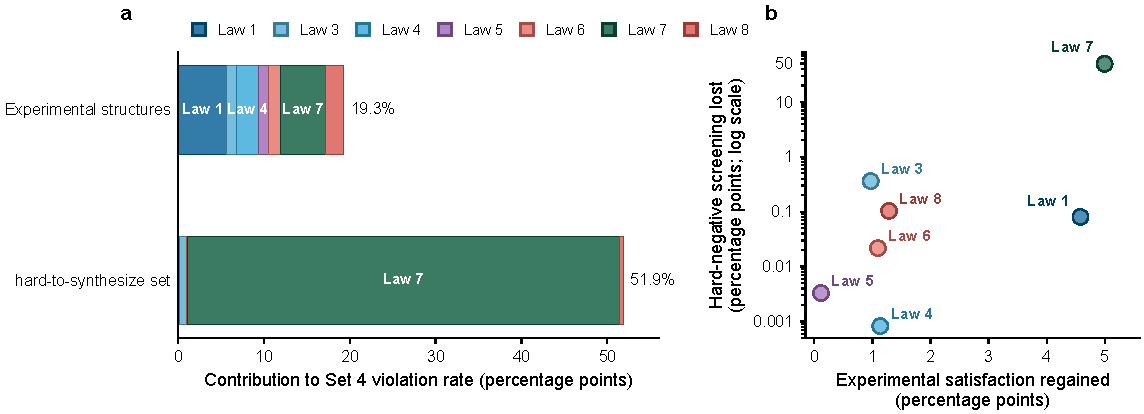
\includegraphics[width=\textwidth]{figs/figS17_l4_contributions.pdf}
  \caption[Law-wise attribution of Set~4 screening]{\textbf{Law-wise attribution of Set~4
  screening in experimental and PU hard-negative structures.} Records without a
  verdict remain in both cohorts.
  \textbf{a},~Stacked bars allocate the Set~4 violation rate among Law~1 and Law~3--Law~8 for the
  deduplicated experimental and PU hard-negative cohorts. Each multi-law violation is
  divided equally among its active laws. \textbf{b},~Each coloured point is a
  leave-one-law-out comparison, with experimental-structure satisfaction regained on the
  horizontal axis and hard-negative screening lost on the logarithmic vertical axis.}
  \label{sifig:l4-contribution}
\end{figure}

\textbf{Two PU representations.} CGCNN-PU is a task-trained crystal graph convolutional
network. MatterSim-1M-MLP-PU uses frozen 128-dimensional representations from the
MatterSim-v1.0.0-1M checkpoint followed by an MLP head, providing a complementary
encoding learned during universal-potential training. Both models were evaluated
across 50 validation bags containing held-out experimental positives and sampled
unlabelled pseudo-negatives. Mean ROC--AUC was $0.976538\pm0.000763$ for CGCNN-PU
and $0.946566\pm0.000942$ for MatterSim-1M-MLP-PU. Each CGCNN-PU bag contained
19{,}798 positives and 19{,}798 pseudo-negatives. MatterSim embedding
availability left approximately 37{,}850 records per bag. Supplementary
Fig.~\ref{sifig:pu-model-performance}a--d shows the mean ROC curves, bag-wise
envelopes, and confusion matrices at the fixed 0.5 decision threshold.

\begin{figure}[!htbp]
  \centering
  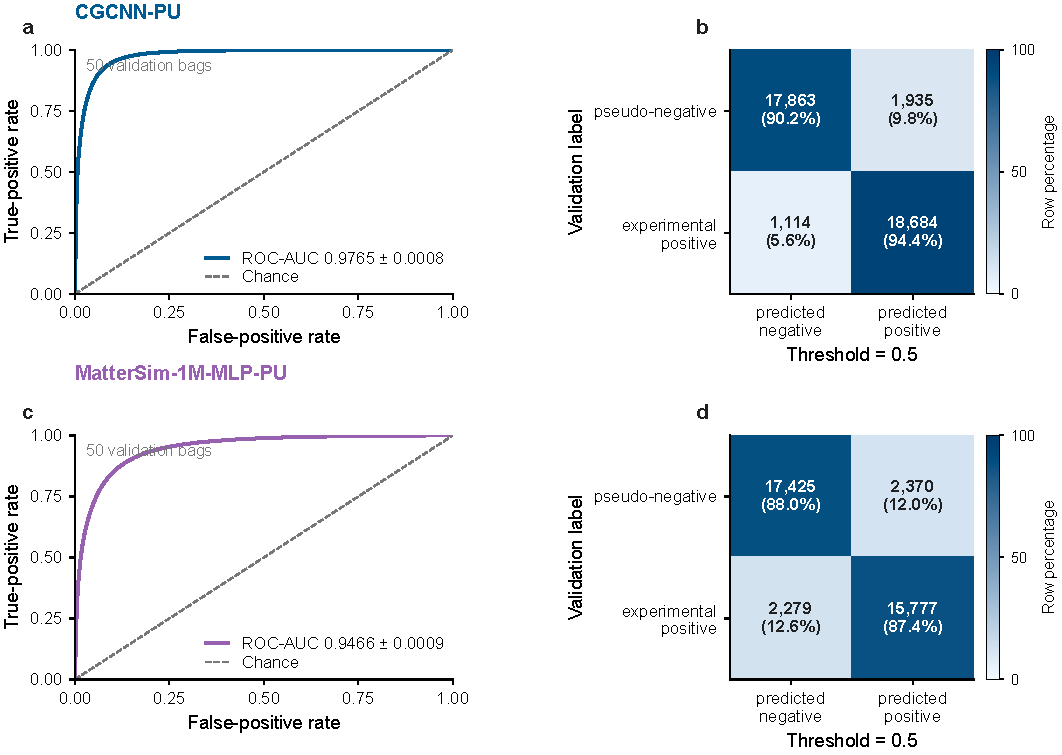
\includegraphics[width=\textwidth]{figs/figS18_pu_model_performance.pdf}
  \caption[Validation performance of the two PU models]{\textbf{Validation performance of
  the two positive--unlabelled learning models.} Every bag contains held-out
  experimental positives and sampled pseudo-negatives.
  \textbf{a,c},~Mean receiver-operating-characteristic curves for CGCNN-PU and
  MatterSim-1M-MLP-PU across validation bags. Axes are false- and true-positive rates,
  shading gives the central bag-wise envelope, legends report the bag-level ROC--AUC
  summary, and the diagonal marks chance. \textbf{b,d},~Confusion matrices at the fixed
  decision threshold. Rows are validation labels, columns are predictions, and cells
  show bag-mean counts and row percentages.}
  \label{sifig:pu-model-performance}
\end{figure}

\begin{figure}[!htbp]
  \centering
  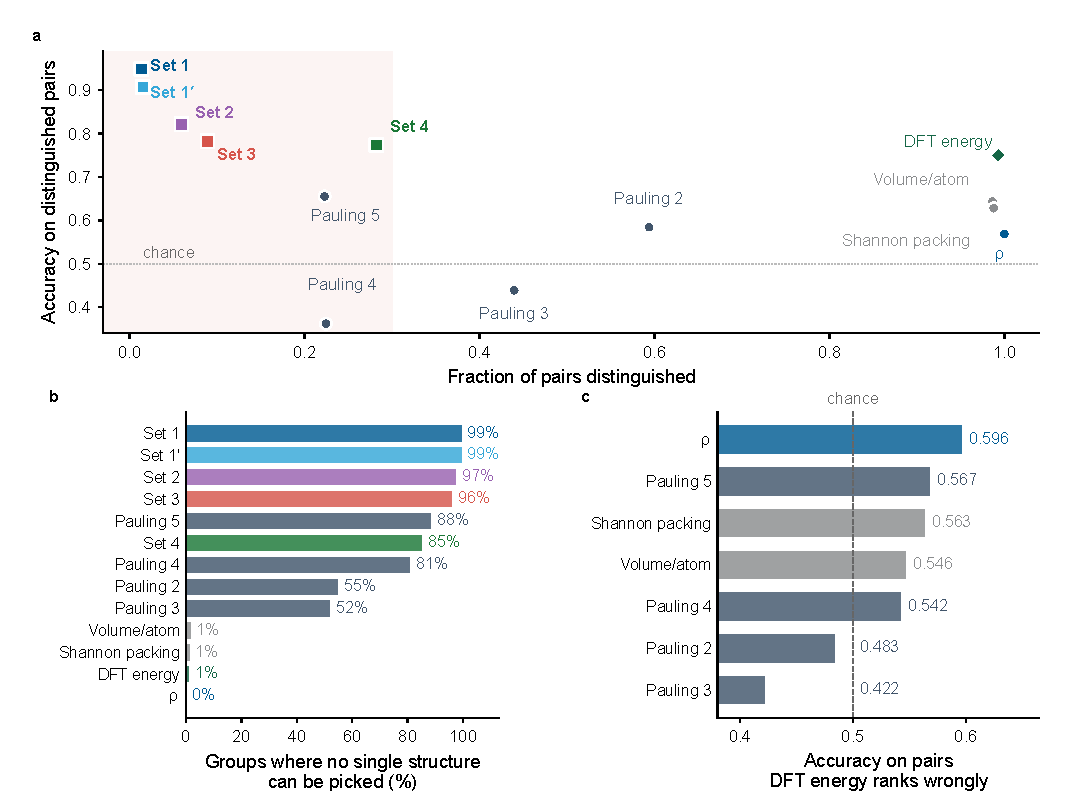
\includegraphics[width=\textwidth]{figs/figS19_polymorph_ranking.pdf}
  \caption[Decision boundaries in same-composition polymorph ranking]{\textbf{Decision
  boundaries in same-composition polymorph ranking.}
  \textbf{a},~The fraction of within-composition pairs distinguished is plotted against
  group-equal accuracy on distinguished pairs. Shapes and colours identify baseline
  criteria, PRIS law sets and DFT energy, and the shaded band marks the low-decision
  region. \textbf{b},~Bars show the fraction of composition groups for which no unique
  structure is selected. \textbf{c},~Bars show non-energy-criterion accuracy on pairs
  ordered incorrectly by DFT \(E_{\mathrm{hull}}\). Ties are excluded from accuracy,
  and horizontal lines mark chance.}
  \label{sifig:polymorph-ranking}
\end{figure}

\begin{figure}[!htbp]
  \centering
  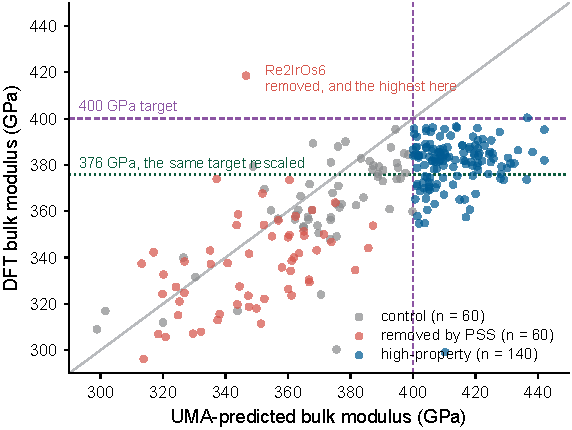
\includegraphics[width=0.72\textwidth]{figs/figS20_dft_e4_bulk.pdf}
  \caption[Property screen against first-principles bulk moduli]{\textbf{The property
  screen against first-principles bulk moduli.} Each point is one candidate. The
  horizontal axis is bulk modulus predicted by the UMA machine-learning model,
  which defined the design target. The vertical axis is the DFT bulk modulus from
  a third-order Birch--Murnaghan fit to a five-point energy--volume curve. The
  plot shows 260 of 261 selected candidates; one cell did not converge. The
  DFT values are a median 0.940 times the machine-learning predictions, so
  the model predicts systematically higher bulk moduli. Thus its 400\,GPa target
  (dashed) maps to 376\,GPa on the DFT scale (dotted).
  Ranking is nevertheless retained: a high-property candidate outranks a removed
  candidate 0.966 of the time. Only three of the 140 highest DFT bulk moduli were
  removed by the screen. Re$_2$IrOs$_6$ is the informative exception: the screen
  removed it, but DFT ranks it highest. This cohort deliberately oversamples high
  machine-learning predictions, so these fractions do not transfer to the full
  candidate pool.}
  \label{sifig:dft-e4-bulk}
\end{figure}

\begin{figure}[!htbp]
  \centering
  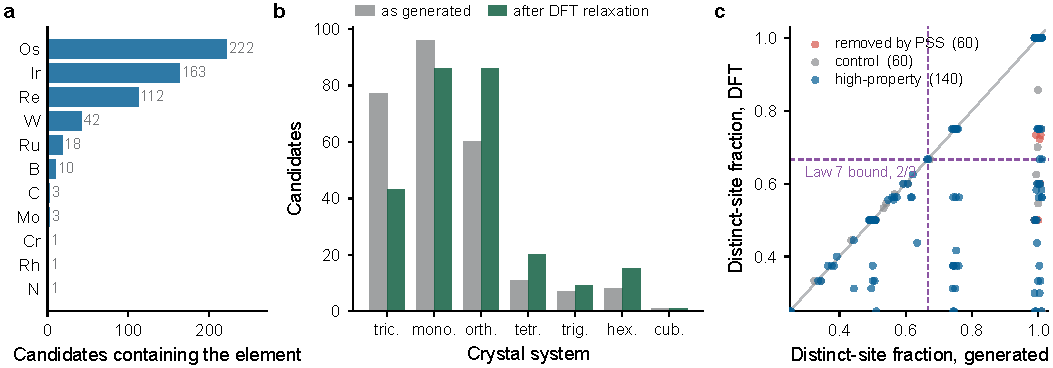
\includegraphics[width=\textwidth]{figs/figS21_dft_e4_composition.pdf}
  \caption[Composition and symmetry of the relaxed design candidates]{\textbf{What the
  property-conditioned queue is made of, before and after relaxation.} The panels
  show all 260 candidates whose bulk moduli were computed. \textbf{a},~Number of candidates containing each
  element. Conditioning on a bulk modulus above 400\,GPa drives the generator into a narrow
  corner of the periodic table, dominated by the 5d transition metals.
  \textbf{b},~Crystal system before and after DFT relaxation. Both use the
  0.01-\AA{} tolerance applied in every Law~7 verdict. \textbf{c},~The Law~7
  distinct-site fraction before and after relaxation. Colour gives the
  synthesizability-screen decision. Points can only fall below the diagonal
  because relaxation merges sites and does not split them. Dashed lines mark the Law~7 threshold of two-thirds on each axis. Relaxed cells are provided as
  Supplementary Data.}
  \label{sifig:dft-e4-composition}
\end{figure}


\textbf{Continuous CLscore relation.} Raw scores from the two models have
different scales and were not averaged directly. Records were first assigned to
ten within-model percentiles. PRIS and PSS summaries were calculated separately,
then averaged pointwise across aligned percentiles. From the lowest to highest
percentile, mean Set~4 violation fell from 50.3\% to 30.4\%, while mean PSS rose
from $-11.37$ to $-0.18$. The shared direction across task-trained and pretrained
representations is the cross-model evidence used in the main text.

\textbf{MatterSim-computed \(E_{\mathrm{hull}}\) threshold.} A separate balanced
pilot sampled 1{,}024 experimental structures and 1{,}024 PU hard negatives.
MatterSim relaxation returned finite energies for 2{,}045 structures. For each
composition, we subtracted the Materials Project phase-hull reference. We then
swept the \(E_{\mathrm{hull}}\) threshold. At 0.20\,eV per atom, the method
retained 86.2\% of the experimental sample and screened 72.0\% of the PU sample.
The energy route therefore requires relaxation and phase-reference construction
beyond direct PRIS evaluation.

\textbf{Property-conditioned inverse-design protocol.} We ran MatterGen v1.0.3
from model-repository commit
\texttt{67afb22ea0dd0073aedfc85b30b94bea0ee21863}. The public bulk-modulus
checkpoint conditioned 13 independently seeded shards at 400\,GPa, yielding
1{,}664 parsed structures.

StructureMatcher deduplication used \texttt{ltol=0.2}, \texttt{stol=0.3}, and
\texttt{angle\_tol=5} degrees. It removed 583 equivalent outputs and left 1{,}081
unique, unrelaxed structures.

The \texttt{uma-s-1p1} checkpoint independently predicted bulk modulus through
its \texttt{omat} energy task. We evaluated energies at fixed fractional
coordinates and five cell volumes from 0.96 to 1.04 times the generated volume.
Each quadratic \(E(V)\) fit had to reach \(R^2\geq0.98\). All 1{,}081 fits passed,
and 140 structures had a clamped machine-learning prediction of at least
400\,GPa.

PSS coefficients and preprocessing remained fixed from Supplementary
Section~\ref{note:s15}. Each generated structure supplied two of six PSS
descriptors; the other four used frozen training medians. We calibrated the
threshold on 541 experimentally recorded structures with the same two-descriptor
support and a valid UMA prediction of at least 200\,GPa. A target satisfaction of
97.5\% selected PSS cutoff $-0.636879$, which retained 528 of the 541 calibration
structures.

Scores below this cutoff were screened, whereas ties were retained. The cutoff
produced 97.6\% satisfaction, removed 61 generated candidates, and retained all
140 high-property candidates. No generated score or property label entered
fitting, preprocessing, or cutoff estimation. The generated queue defined only
the matched two-descriptor support stratum. Within this stratum, the frozen score
reduces exactly to
\begin{equation*}
  \mathrm{PSS}=5.597386-3.133285\,\eta_{\mathrm{site}}
  -0.206563\,v_{\mathrm{atom}}.
\end{equation*}
All 61 screened structures had \(\eta_{\mathrm{site}}=1\), passed both the 0.5-
and 0.7-\AA{} distance cutoffs, and violated Law~7. Their volumes ranged from
15.017 to 16.558\,\AA$^3$ per atom, with mean 15.329\,\AA$^3$. The retained queue
had mean 14.331\,\AA$^3$ per atom. The PSS-screened structures were a strict
subset of the 728 Set~4 violations. Set~4 also removed 95 of the 140
high-property candidates, whereas denser packing kept them above the continuous
PSS threshold.

The matched Ir$_2$Os$_7$ examples in the main figure make this distinction
concrete. The screened P1 structure has 18 inequivalent sites among 18,
\(v_{\mathrm{atom}}=15.017\)\,\AA$^3$, and \(\mathrm{PSS}=-0.638\). The retained
C2/m structure has four inequivalent sites among nine,
\(v_{\mathrm{atom}}=14.327\)\,\AA$^3$, \(\mathrm{PSS}=1.245\), and a UMA-predicted
bulk modulus of 408.7\,GPa.

Generation manifests, model hashes, and the deduplicated archive are preserved
as generation/model artefacts. Evaluation tables and the final support-matched
evaluation are preserved as analysis artefacts.

\section{Extending the plausibility sequence with structural simplicity and bond valence}\label{note:s17}\label{si-note:s17}

\textbf{Pre-registration.} The Set~4 plausibility plan was fixed before the
augmented matrix features or any law search existed. Its SHA-256 was recorded in
the repository. The analysis reused audited, reserve-free tables containing
17,929 experimental and 12,202 damaged structures. Damaged structures were
recreated with the pipeline's original seeds. Before search began, Set~3 was
reproduced to all four published decimals on both splits.

The model class kept Set~3 unchanged and allowed at most four added laws. Each
addition had to be expressible as a one-line physical statement. Candidate
thresholds came from a fixed percentile grid of the experimental discovery
distribution. This produced 8{,}466 candidate laws over 94 structural quantities
that met the inclusion criteria. Greedy selection maximised discovery damage
detection while requiring experimental satisfaction of at least 0.81.

The prespecified script evaluated the held-out split once. Its earlier repeated
use is disclosed in Section S8.

\textbf{Selection.} The search stopped at its prespecified minimum required gain after two additions:
\begin{itemize}
\item \textbf{Law~7 (simpler-structure law):} the fraction of
crystallographically inequivalent sites is at most $2/3$. This writes Pauling's
preference for simpler structures as a threshold law. The threshold is the
90th-percentile grid point of the experimental discovery distribution, or about
the 92nd percentile of structures.
\item \textbf{Law~8 (bond-valence deviation):} the mean relative deviation of
bond-valence sums from nominal valences is at most $0.7143$. This hard threshold
expresses the electrostatic valence principle.
\end{itemize}
On discovery data, satisfaction was 0.8107 and damage detection was 0.9051. A
third candidate improved detection by only 0.0035. This gain was below the
pre-registered minimum, so selection stopped.

\textbf{On held-out data.} Satisfaction was 0.8180 and overall damage detection
was 0.9111. Detection by type was 0.7338 for D1, 0.9091 for D2, 1.0000 for D3,
0.9288 for D4, and 0.9851 for D5. Of 5{,}297 experimental structures, 3{,}713
satisfied Set~4, 964 failed at least one law, and 620 received no verdict. Of
3{,}612 damaged structures, 237 satisfied Set~4, 3{,}291 failed at least one law,
and 84 received no verdict. All three pre-registered criteria were met:
satisfaction $\geq0.80$, damage detection $\geq0.80$, and no type below 0.55.
The lowest type-specific detection exceeded its required minimum by 0.18.

\textbf{Testing on one damage type omitted during fitting.} The five unseen-type
detection rates were 0.7243 for D1, 0.8924 for D2, 1.0000 for D3, 0.7928 for D4,
and 0.6863 for D5. The folds omitting compression, cation--cation swap, or
displacement selected the same two laws at the same thresholds. The folds
omitting expansion or cation--anion swap selected different additions. They
still reached 0.79 and 0.69 detection on their unseen types, respectively. This
behaviour is consistent with physicochemical laws rather than one
perturbation-specific pattern.

The 0.2318 result for the provably optimal depth-3 tree is not a direct
comparison. This test refits additions on top of fixed Set~3, whereas the tree
was refitted in full.

\textbf{A further evaluation population.} Without refitting, we applied Set~4 to
the main-text Fig.~4a,b benchmark. It contains 440 experimental parent structures
and 2{,}024 damaged counterparts generated with the Section S12 operators. The
parents came from the analysis set. Counts across the three partitions were
259/115/66, so this population is not disjoint from the search splits.

Set~4 achieved satisfaction 0.8295 and damage detection 0.8790. Type-specific
detection was 0.7295 for D1, 0.8636 for D2, 1.0000 for D3, 0.8045 for D4, and
0.9909 for D5. These values are consistent with the held-out result. Overall
detection was 27 times that of the 0.7-\AA{} filter on the same structures.
Per-structure results accompany the figure source data.

\subsection{Preference for simpler structures and bond valence detect different failure types}

Applied singly on top of fixed Set~3, the additions divide the work. This is a
descriptive decomposition of the published Set~4 evaluation, not a new success
test. Set~3$+$Law~7 achieved held-out satisfaction 0.8361 and damage detection
0.8696. Its D1--D5 rates were 0.678, 0.899, 1.000, 0.788, and 0.984. Set~3$+$Law~8
achieved satisfaction 0.8964 and detection 0.7622. Its corresponding rates were
0.687, 0.596, 0.960, 0.915, and 0.609.

Law~7 provides most of the gain for swaps and displacements. Law~8 improves
expansion detection and gives smaller improvements elsewhere. Law~7 detects
nearly every perturbation that breaks crystallographic equivalence, but few other
damaged structures. R5 identified the same class sensitivity when symmetry was
tested alone. Within Set~4, other laws detect the classes Law~7 misses. The
combined model provides a numerical form of Pauling's fifth rule. The
experimental merge control below confirms that merging does not generally erase
distinct sites in experimental structures.

Law~7 also depends on a symmetry tolerance. Site orbits are identified on the
as-given cell with spglib at \texttt{symprec=0.01}. Increasing this tolerance to
0.1 changes verdicts for only 0.15 per cent of experimental and 0.26 per cent of
damaged structures. The law presumes symmetrised input; structures with
refinement noise should first be symmetrised.

When D5 was omitted, the refit selected a related symmetry law, space-group
number $\geq2$, rather than Law~7 itself. Thus the data repeatedly select the
symmetry and distinct-site family, not one exact threshold.

\subsection{The bond-valence law isolates extreme values}

Across 10{,}725 experimental discovery rows with finite values, mean relative
bond-valence deviation had median 0.094, upper quartile 0.200, ninetieth
percentile 0.524, and ninety-fifth percentile 0.682. The fixed threshold 0.7143
is the 96th-percentile grid point. The same rows had median global instability
index 0.215 valence units, close to the $\sim0.2$ v.u. convention in bond-valence
practice.

Law~8 is therefore a deliberately permissive upper-tail bound, not a
working-chemist's quality criterion. Its discrimination comes from distribution
separation. Across finite discovery and held-out rows, the medians were 0.094 for
experimental and 0.705 for damaged structures. The law excludes the extreme tail where damaged structures concentrate.
Rows with no computable bond-valence parameters (2{,}698 of 17{,}929) satisfy Law~8
automatically under the missing-value convention of Section~\ref{s3.3-missing-values}.

\subsection{The physical families recur across search settings}

The prespecified greedy search was repeated at required satisfaction values 0.75,
0.78, 0.81, 0.84, and 0.87. Discovery damage detection remained between 0.85
and 0.95 throughout. High detection is therefore not an artefact of the 0.81
requirement, which primarily sets satisfaction.

The exact Law~7$+$Law~8 pair appeared only at 0.81. At 0.78 and 0.84, the search
again selected the Law~8 quantity, but at a tighter threshold. At three of the
four other satisfaction levels, a space-group law replaced Law~7. This
recurrence identifies a symmetry and distinct-site family rather than one fixed
threshold.

When all Pauling-derived families were excluded, contact and charge-topology
laws still achieved 0.8655 detection at the same satisfaction. This retains
about 80 per cent of the gain over Set~3. The excluded features comprised Wyckoff,
space-group, bond-valence, and rule-2/4/5 quantities. When only symmetry features
were excluded, detection reached 0.8810 and the bond-valence family was selected
first.

Pauling-derived families are therefore not necessary for high damage detection
on this suite. A free search nevertheless selects them first, and they provide
the final improvement.

\subsection{The full law-set sequence preserves its advantage at matched satisfaction}

The 27-fold margin over the 0.7-\AA{} filter compares settings with different
satisfaction. For a matched comparison, an absolute cutoff of 1.71\,\AA{} was
tuned to Set~4's 83.0 per cent satisfaction. It detected 0.339 of damaged
structures, compared with 0.879 for Set~4, a 2.6-fold margin. The corresponding
matched-satisfaction margin for Set~1 was 2.1-fold.

The parent-cluster bootstrap interval for Set~4 satisfaction was
$[0.793,0.864]$, centred at 0.830. Its damage-detection interval was
$[0.864,0.894]$, centred at 0.879. Among 66 reserve-partition parents,
satisfaction was 0.879 and damage detection was 0.909. The 0.7-\AA{} baseline
detected 0.026. These reserve-parent values are not an untouched reserve test,
because the S8 split-labelling error exposed part of the wider reserve to a
full-sample threshold fit.

\subsection{The law-set sequence responds smoothly to increasing perturbation amplitude}

The Section S12 benchmark uses one amplitude per damage type. We therefore repeated
three perturbations at graded amplitudes on the same 440 parents (Supplementary
Fig.~\ref{sifig:amplitude}). The PRIS sequence begins responding near 10 per cent
strain and 0.1\,\AA{} displacement. By contrast, the fixed 0.5- and 0.7-\AA{}
distance filters remain near zero detection below 0.4\,\AA{} displacement.

Under Gaussian displacement, Law~7 reaches 1.00 detection by 0.05\,\AA{} because
any Cartesian noise breaks Wyckoff degeneracy. The simpler-structure law thus
responds first at small amplitudes. Set~1--Set~3 show a progressive response over
the same range.

\subsection{Law sets fixed before evaluation separate generator outputs beyond distance filters}

The analyses above contain no generative-model samples. We therefore asked
whether the fixed law sequence separates raw generator outputs beyond distance
filters. The sample comprised 500 MatterGen structures from the deposited,
seeded seven-generator benchmark below. Every structure satisfied both fixed
absolute-distance filters at 0.5 and 0.7\,\AA{}.

Across all 500 outputs, the fractions receiving a verdict and satisfying each
set were 32.4 per cent for Set~1, 30.8 per cent for Set~2, 26.8 per cent for
Set~3, and 0.8 per cent for Set~4. No-verdict cases remain in these denominators
but are not classified as failures. For Set~3, 134 structures satisfied the set,
11 failed it and 355 received no verdict.

Even with the mean-valence fallback, 338 structures had no charge assignment.
Among 162 charge-assignable structures, 4 satisfied Set~4, 155 failed it, and 3
had no verdict because another measurement was unavailable. None of the 162
failed the reduced-distance law. The later separation therefore comes
from chemical, electrostatic, and site-order laws.

These raw outputs have no DFT results, so law satisfaction does not establish
correctness. The interatomic-potential analysis below provides an energy check.
Charge assignment remains the primary limit on verdict coverage for new
structures.

\subsection{The distinct-site law exposes excess site complexity in a public generative
release}\label{si-note:s17-gnome}

\textbf{Protocol fixed before computation.} We downloaded all 554{,}054 structure
files in the public GNoME stable-structure release from its official repository.
Before parsing any structure, a written protocol fixed the seed for a uniform
sample of $N=5{,}000$.

For each primitive cell, spglib identified site orbits at
\texttt{symprec=0.01}. The deposited space-group label was never used in the
verdict. This primitive-cell convention differs from the as-given-cell convention
in the discovery tables. Absolute external Law~7 rates, and Set~4 rates containing
Law~7, are therefore descriptive rather than directly comparable with the
discovery rate. Every sampled structure was parsed and analysed for symmetry.

\textbf{Result.} Law~7 was not satisfied by $2{,}032/5{,}000=40.6\%$ of the
sample. By deposited label, failure rates were 100\% for P1 (727/727), 96.6\% for
Pm (731/757), and 88.4\% for Cm (305/345). Rates were 16.6\% for Amm2, 1.4\% for
C2/m, and 7.7\% for all other groups pooled.

Orbit detection might assign higher symmetry than the deposited label and
thereby change verdicts, especially for P1. We therefore repeated the analysis at
the tenfold coarser \texttt{symprec=0.1}; the failure rate changed by less than
one percentage point, to 39.7\%. At the primary tolerance, spglib assigned a
strictly higher group than the deposited label for only 0.02\% of the sample and
agreed with the label for 97.5\%.

Failures are therefore concentrated in P1, Pm, and Cm, quantifying the release's
published space-group anomaly. The sample's median distinct-site fraction is
0.60, compared with the experimental 90th-percentile
threshold of $2/3$. The
protocol, per-structure table, and summary are archived.

\textbf{The similar-element merge test.} The over-ordering hypothesis is that
the release assigns chemically similar atoms to distinct crystallographic sites.
If so, merging same-group elements should restore symmetry in Law~7 failures.
By contrast, merging should have less effect when chemically distinct sites are
also geometrically distinct.

We drew a stratified sample of 300 entries from the fixed 5{,}000 structures.
It contained 150 Law~7 failures, stratified over P1, Pm, Cm, and remaining groups,
and 150 structures satisfying Law~7. Elements in the same periodic group were
merged, with Sc, Y, and the lanthanides treated as one class. We then recomputed
orbits and space groups under the same convention.
At least one same-group pair was mergeable in 113/150 Law~7 failures and 78/150
structures satisfying Law~7. At the strict 0.01-\AA{} tolerance, merging changed
little because relaxed geometries lie off ideal sites. We therefore used the
0.1-\AA{} tolerance, at which the whole-sample Law~7 failure rate changes by less
than one percentage point.

Among mergeable Law~7 failures, 78\% moved to a distinct-site fraction of $2/3$
or below and 79\% moved to a higher space group. The median space group rose from
Pm (no.\,6) to Pnma (no.\,62). Non-mergeable failures were unchanged, with median
distinct-site fraction 1.0 before and after. Structures already satisfying Law~7
shifted only modestly. In this stratified sample, the intervention supports
near-symmetric lattices carrying ordered labels for chemically similar elements.

An experimental control used 12{,}000 random structures. Only 27 both failed
Law~7 at the same tolerance and contained a mergeable same-group pair. The
identical protocol restored higher symmetry for none of them (0/27), and median
distinct-site fraction remained 0.80. Experimental oxysulfides, oxyfluorides,
and mixed alkalis place same-group elements on geometrically distinct sites, so
relabelling cannot erase them. The restoration in the generative sample is thus
not explained by the merge operation alone and is consistent with its
element-label assignments.

A complementary database search found a disordered ICSD entry with the identical element
set for only 2 of 300 sampled entries. This is consistent with the release's novelty
criterion. The intervention is therefore the direct test, rather than a database
lookup.

\subsection{Bond-valence and chemical-order laws dominate failures in the assignable subset}

A second protocol fixed the sample and verdict procedure before all eight laws
were applied to the same 5{,}000 structures. A final audit found that the external
Law~8 implementation did not reproduce the discovery definition. We recomputed
Law~8 with the discovery analysis's CrystalNN graph and tabulated bond-valence
parameters. The original protocol, code, and outputs remain preserved.

Charge assignment first sought integer charge balance. If that failed, it used
non-integer mean valences. Structures for which both methods fail receive no
verdict and are never counted as failures. Charges were assigned to 376 structures,
or 7.5\% of the sample. The remainder is largely intermetallic and outside the
stated domain. Within the assignable subset, individual contact and electrostatic
laws had 94.7--99.2\% satisfaction, as expected for a DFT-relaxed release.

\begin{center}
\begin{tabular}{lrrrr}
\hline
law set & evaluable & satisfy & fail & no verdict \\
\hline
Set~3 & 335 & 281 & 54 (16.1\%) & 41 \\
full Set~4 & 314 & 159 & 155 (49.4\%) & 62 \\
\hline
\end{tabular}
\end{center}

Counts are relative to the 376 charge-assigned structures; percentages in the fail column
use the evaluable denominator. Of the 155 full-set failures,
88 (56.8\%) satisfied Set~3 but failed Law~7 or Law~8: 41 failed Law~7 alone,
17 failed Law~8 alone, 14 failed both, and 16 failed Law~7 while Law~8 was
unavailable.

Law~8 was evaluable for 254 structures, or 67.6\% of the charge-assignable
subset, because coverage is limited by bond-valence parameters. It failed for 36
of these 254 structures (14.2\%). Law~7 failed for 26.1\% of the
charge-assignable subset, compared with 40.6\% of the full sample. The
charge-assignable subset is more symmetric than the intermetallic-dominated
remainder, and the two rates have different denominators.

\subsection{Symmetry-aware generators better preserve the distinct-site fraction}

The pre-analysis protocol extended the MatterGen sample to seven public
generative models and one experimental control. Structures came from the openly
licensed WyckoffTransformer benchmark deposit (CC BY 4.0). We sampled 500
structures per model at a fixed seed. The control comprised 500 structures from
the MP-20 test split, the standard generative benchmark of Materials Project
cells containing at most 20 atoms.

The fixed absolute-distance filters had 91--100\% satisfaction for every model's
raw outputs and did not separate generators from the control. The law sequence
did. Formal-charge requirements prevented a verdict for 66--76\% of generator
outputs and 57\% of the intermetallic-heavy control.

Among charge-assignable outputs from coordinate-generating models without
explicit symmetry constraints (MatterGen, DiffCSP, and MiAD), 0--2.5\% satisfied
Set~4. For symmetry-constrained models (DiffCSP++, CrystalFormer, SymmCD, and
WyckoffTransformer), 29.9--46.1\% satisfied Set~4. The experimental control rate
was 64.3\%. Structures missing another required measurement received no verdict
and were excluded from these rates.

At the strict tolerance, Law~7 failed for 95--100\% of raw structures from
models without imposed symmetry, where nearly every atom was inequivalent.
Per-structure tables and implemented thresholds are archived separately from the
deposit checksum.

\textbf{Robustness checks: full denominators and relaxation.} First, each
Set~4 rate above uses a model-specific charge-assignable subset. Law~7 requires
no charges and can be evaluated on every raw output. On full 500-structure
denominators, it failed for 96--100\% of cells without explicit symmetry, 24--28\%
of symmetry-constrained cells, and 27\% of controls. This reproduces the same
separation and rules out charge coverage as its cause.

Second, numerically triclinic, unrelaxed outputs could make orbit detection
sensitive to coordinate noise. We therefore relaxed 2{,}500 structures from
MatterGen, DiffCSP, MiAD, SymmCD, and the experimental control. The prespecified
MatterSim protocol is given in the relaxation-energy subsection below. Law~7 was
then recomputed at \texttt{symprec=0.1} to tolerate residual numerical noise.

After relaxation, Law~7 failure was 65.0\% for MatterGen, 67.0\% for DiffCSP,
40.2\% for MiAD, 30.0\% for SymmCD and 26.0\% for the experimental control;
relaxation left the last two unchanged. Thus relaxation
reduces but does not erase the Law~7 separation in these tested sets. Numerical
noise in unrelaxed coordinates cannot explain the entire signal. This local
MatterSim check does not establish experimental stability or a universal
property of generators without explicit symmetry constraints.

\subsection{Crystal-chemistry laws complement coordinate-based validation}

checkCIF/PLATON requires diffraction data, displacement parameters, and
refinement fields unavailable here. We therefore did not run the established
software. A protocol fixed before computation reimplemented only the four test
families calculable from atomic coordinates and a unit cell:
\begin{enumerate}
\item missed higher symmetry, when spglib at 0.3\,\AA{} returns a higher group
than at 0.01\,\AA{};
\item short non-bonded contacts, when a non-covalently bonded pair lies below
0.85 of the van der Waals radius sum, with 0.75 and 0.95 as sensitivity values;
\item solvent-accessible voids, measured with a 1.2-\AA{} probe on a 0.5-\AA{}
grid and flagged above 5\% of cell volume, with 2\% and 10\% as sensitivity
values; and
\item floating atoms, defined by no neighbour within 1.3 of the covalent radius
sum.
\end{enumerate}
These are coordinate-based reimplementations; no checkCIF/PLATON alert code is
claimed or matched.

A final audit found that the external Law~8 calculation did not reproduce the
discovery definition. We recomputed the values with the discovery CrystalNN graph
and tabulated bond-valence parameters. The original protocol, code, and outputs
remain preserved.

For the six-law comparison, each parent and damaged counterpart was converted to
a primitive cell before Law~7 evaluation. Paired comparisons therefore share a
cell convention. Their absolute Law~7 rates are not directly comparable with the
deposited-cell discovery tables.

We took the first 300 entries with composition-only integer charge assignments
from a seed-shuffled scan of 8{,}000 public generative structures. This enriched
sample cannot estimate population charge coverage. In the uniform 5{,}000
sample, 222 structures (4.44\%) had integer assignments.

Each parent was perturbed once per applicable Section~\ref{note:s12} damage type.
Computed parent crystals served as controls because the experimental coordinates
are not redistributable. The four-check set failed for 0.303 of parents, and the
six-law PRIS set failed for 0.507. After observing these parent rates, we added a
paired analysis. A damaged structure counted as detected only when its parent
satisfied the same method.

The six-law set comprises Law~1 and Law~4--Law~8. In this sample, Law~7 and Law~8
failed for 0.257 and 0.178 of parents. These values are comparable with 0.261 and
0.142 in the 376 charge-assignable structures above.

\begin{center}
\begin{tabular}{lccccc}
\hline
paired damage detection & D1 & D2 & D3 & D4 & D5 \\
\hline
missed higher symmetry & 0.003 & 0.045 & 0.000 & 0.000 & 0.000 \\
short non-bonded contacts & 0.507 & 0.148 & 0.621 & 0.247 & 0.397 \\
solvent-accessible voids & 0.000 & 0.000 & 0.000 & 0.037 & 0.000 \\
floating atoms & 0.000 & 0.031 & 0.030 & 0.409 & 0.097 \\
\textbf{four checks together} & 0.512 & 0.215 & 0.622 & 0.522 & 0.431 \\
\hline
Law~7 distinct-site fraction & 0.135 & 0.833 & 1.000 & 0.000 & 0.964 \\
Law~8 bond valence & 0.353 & 0.336 & 0.831 & 0.950 & 0.124 \\
\textbf{six-law set} & 0.697 & 0.892 & 1.000 & 0.936 & 0.982 \\
\hline
\end{tabular}
\end{center}

The pre-specified comparison included structures for which both methods returned
a verdict. PRIS alone detected 0.365, whereas the four checks alone detected
0.021. The post-result paired comparison additionally required the parent to
satisfy both methods. The corresponding fractions were 0.430 and 0.042.

The coordinate-based symmetry check asks whether a looser tolerance reveals
higher symmetry than the tight-tolerance assignment. It detected few wrong-site
exchanges because it was not designed specifically for them. Law~7 instead asks
whether the number of distinct site orbits is implausibly high.
The unrestricted sample, both sensitivity sweeps and the per-structure table are
archived with the analysis records.

\subsection{The laws return no verdict outside their domain and detect anomalies in the evaluable falsified depositions}
\label{s17.x-realworld}

The comparison above evaluates damage introduced by our perturbation procedures. We therefore evaluated a
historical collection of falsified structures that was not created for this benchmark,
without refitting any threshold. The primary source is Harrison et al. (2010), cited in
the main text.

\textbf{The 2010--2012 falsified depositions.} Our recovered archive contains
184 structure reports listed across seven retraction notices
\cite{iucr2010retractionzhong,iucr2010retractionliu,iucr2010retractionapril,
iucr2011retractionmarch,iucr2011retractionoctober,iucr2012retraction,iucr2012retractionjuly}.
Harrison et al. describe reuse of bona fide intensity data after changing one or
more atoms, sometimes with cell adjustments below 4\% and deleted reflections.

For 181 reports, the archive lacks structure-specific true-parent or
substituted-element provenance. We therefore do not infer which depositions share
one diffraction dataset. We retrieved all 184 supplementary CIFs from the
journal archive because COD removes coordinates from retracted entries. Of
these, 177 parsed successfully.

Molecular coordination compounds dominate the corpus and largely lie outside the
laws' domain. No formal-charge assignment was available for 172/177 parsed
depositions (97.2\%); these receive no verdict. The one available original
control exceeded the evaluation size cap and also received no verdict. These are
the stated domain boundaries. All five evaluable depositions failed the laws.

Four evaluable records share an M(C$_2$H$_2$N$_3$Cl) ligand framework and label
M as Cu, Ni, Mn, or Fe in separate papers \cite{iucr2012retraction}. This grouping
does not establish a common genuine parent. All four violate the same two laws.
Their shortest contact has $\rhoc=0.53$, in the strongly repulsive range because
the assigned ionic radius is incompatible with the bond lengths. Mean
bond-valence deviation is 0.77--0.78, above the 0.7143
threshold. The pattern matches
the main-text cation-swap mechanism in falsified depositions rather than
controlled damage.

The fifth evaluable structure, KNOF$_2$, fails the stricter reduced-distance
law at $\rhoc=0.79$. Retrieval records and verdicts are archived separately
from the retraction-notice list.

\subsection{Relaxation energies provide an independent check on damage severity}

A pre-analysis protocol used the MatterSim v1.0.0-5M machine-learning potential
with fixed cells and FIRE optimisation. Force convergence was
0.05\,eV\,\AA$^{-1}$ with a 200-step cap. Every relaxation converged or reached
the cap.

First, seed 20260815 selected 150 random GNoME parents and counterparts produced
by the paper's perturbations. Parents moved a median 0.03\,\AA{} and released less
than $10^{-3}$\,eV per atom. Median releases were 0.22 eV per atom for compression,
1.10 for expansion, and 6.05 for displacement. Expansion is a lower bound because
the cell remained fixed and one third of runs reached the cap. Swap classes have
only $n=3$ and $n=4$, because just 4/150 intermetallic-heavy parents received a
charge assignment.

Second, a dated addendum fixed the MatterGen protocol before any energy was
computed. All 162 charge-assignable structures satisfied Law~1 and released
median 0.007\,eV per atom (interquartile range 0.002--0.029; median maximum
displacement 0.08\,\AA{}). The 338 structures without charge assignments released
median 0.006\,eV per atom (0.000--0.022).

Because every structure satisfied Law~1, the MatterGen sample cannot measure
false failures or energetic separation. It supports only similarly small
relaxation energies in Law~1-satisfying and no-verdict groups. The separate
parent-versus-damage experiment tests perturbation severity.

\subsection{Composition and structure screens detect different failures}
\label{s17.x-incumbents-scored}

The comparisons above use minimum-distance filters because generative pipelines
apply them as structural tests. Their reported validity metric also contains a
composition test, which we evaluated on the same 440-parent benchmark. In the
CDVAE lineage and LeMat-GenBench suite, this component combines SMACT-style
charge neutrality and electronegativity.

Using \texttt{smact} 4.0 with default settings, 76.8\% of experimental parents
satisfied the composition test. It is therefore stricter on experimental
chemistry than the reduced-distance law. All five perturbations preserve
composition, however, so each damaged structure receives its parent's
composition verdict. Conditional on a satisfying parent, measured damage
detection was 0.000 for every damage type. Composition and structure screens
therefore detect different failure classes. Per-structure results and the run
protocol are archived with the source data.

\textbf{The trade-off, stated plainly.} Set~4 satisfaction is 0.818 on held-out
experimental structures, and Law~7 concentrates much of the loss on low-symmetry
structures. Set~4 therefore suits pipelines that prioritise damage detection; it
does not replace Set~1--Set~3. Law-set choice remains a trade-off between
satisfaction and damage detection, now published up to $(0.8180,0.9111)$.

\section{Robustness and implementation details}\label{note:s18}

This note retains quantitative details that the main text
summarises in one sentence each.

\subsection{The reduced-distance law follows a repulsive tail, not a physical constant}

The left tail of the \rhoc{} distribution over 12{,}601 experimental structures is
steeper than exponential. Over $\rhoc \in [0.41, 0.93]$, a quadratic fit to the log
density reduces the residual sum of squares from $11.82$ to $4.31$ and has positive
curvature $+25.7$. This shape is characteristic of a repulsive wall.

The threshold $0.735$ is the first percentile of the distribution, not a measured
constant. A sweep shows no sharp transition near it: satisfaction is $0.9929$ at
$\tau=0.70$, $0.9900$ at $0.735$, $0.9876$ at $0.75$ and $0.9728$ at $0.80$.
Across the ten commonest anion families, Set~1 satisfaction remains at least $0.981$.
Phosphides are the exception in damage detection, which is $0.0330$ compared with
$0.27$--$0.32$ elsewhere, although all 551 experimental phosphides satisfy the lower
threshold. Thus, for phosphides, the law preserves experimental-structure satisfaction but
contributes little damage detection. Satisfaction among DFT-relaxed candidates is
$0.002$ below that of experimental structures, so relaxation does not inflate it.

\subsection{Provably optimal trees perform well on seen damage types but lose performance on omitted types}

At cost ratio $2.5$, the provably optimal depth-three tree reaches satisfaction $0.9518$
and damage detection $0.6732$. The corresponding values for the four-law core on the
same split are $0.9511$ and $0.6173$. Cost ratios from $1.75$ to $2.25$ return the same
operating point. Replacing accuracy with f1-score also returns the same tree. Thus, within
this search, only the cost ratio moves the trade-off curve. Depth 4 consumed 549\,s
without proving optimality, so every optimality claim is restricted to depth $\leq 3$.

When one damage type is omitted during fitting, the tree's mean damage detection falls
from $0.6712$ on the fitted types to $0.2318$ on the omitted type. A single \rhoc{}
threshold selected by the same procedure reaches $0.2771$ on the omitted type. Its five
signed changes are $-0.140$, $+0.029$, $+0.762$, $-0.336$ and $-0.339$, so their mean
conceals cancellation. Mean absolute change is $0.506$ for the tree and $0.321$ for the
threshold. The tree nevertheless performs better on three of the five omitted types.
The aggregate and per-type comparisons therefore describe different aspects of the
result and must be read together. At satisfaction $0.95$, the depth-three tree does not
select \rhoc{}. Instead, it uses coordination-eccentricity and
site-Madelung-energy-range features, whose held-out damage detection differs by damage
type.

\subsection{Energy span and dominance by one composition reshape cross-database accuracy}

The median intra-composition energy span is 25\,meV per atom in the Materials Project
experimental set, 99 in ELEMENTA, 186 in Alexandria and 449 in LeMat. A method evaluated
on LeMat therefore orders structures separated by approximately 18 times more energy
than those in the Materials Project set. Within the matched
$[50, 200)$\,meV-per-atom window, group-equal accuracies are $0.6912$, $0.6323$,
$0.6287$ and $0.5987$ for MP, ELEMENTA, Alexandria and LeMat, respectively. This
restriction reverses the unmatched ranking (Supplementary
Fig.~\ref{sifig:ranking-data}a,b).

Silica supplies $0.5932$ of pairs in the MP experimental set and $0.4358$ in the
synthesis-target set. By contrast, the largest-group shares are $0.0283$, $0.000358$
and $0.0000631$ in the three computational sets. With pair weighting, density outranks
formation energy, $0.7103$ versus $0.6476$. Equal weighting of composition groups reverses
the order to $0.6347$ versus $0.7451$, which refutes claim R9. Cross-database accuracy
must therefore be reported with its energy window. Pair-weighted results on concentrated
sets must also be accompanied by the largest-group share.

We later analysed all 1{,}508 groups descriptively, rather than as a new held-out test.
With equal weight per group, the fixed PSS scored $0.726$ on the full set. It also scored
$0.726$ after excluding SiO$_2$ and $0.726$ after excluding every tetrahedral-framework
oxide family containing Si, Al, P, Ge or B. Thus, this diagnostic is unchanged when
silica or framework oxides are removed. Bare volume per atom scored $0.643$ under all
three conditions. The experimentally recorded member was denser in 66 per cent of the
1{,}507 non-silica groups. The same direction persisted in non-oxide chemistries
($0.61$).

\textbf{A further robustness check on experimentally recorded structures.} Excluding the 15
composition groups whose every experimental member is recorded in ICSD only
under high pressure leaves the development accuracy of the fixed PSS
unchanged ($0.754$ against $0.755$), so the density term is not driven by
high-pressure phases in the experimentally recorded class.

\subsection{Binary law sets often return ties where continuous scores can rank}

Applied to synthesis ranking as binary criteria, the four law sets give the following
coverage and conditional accuracy:

\begin{center}
\begin{tabular}{lcccc}
\hline
criterion & \shortstack{pair decision\\rate} & \shortstack{groups without\\a unique choice} &
\shortstack{contributing\\groups} & \shortstack{conditional\\accuracy} \\
\hline
Set~1 & 0.0133 & 99.4\% & 39 & 0.9487 \\
Set~1$'$ & 0.0152 & 99.3\% & 43 & 0.9070 \\
Set~2 & 0.0594 & 97.4\% & 156 & 0.8216 \\
Set~3 & 0.0892 & 96.0\% & 225 & 0.7822 \\
\hline
\end{tabular}
\end{center}

Returning a tie is appropriate for a plausibility filter. Thresholding removes the
ordering needed for ranking, which is why the main text treats \rhoc{} as a continuous
quantity for that task.

\subsection{The laws and fitted scores as equations}

The eight PRIS laws are written below exactly as applied in main-text Fig.~1d. Here,
$\rhoc{}$ is the reduced contact ratio from main-text equation (1), and
$f_{\mathrm{i}}$ is the Pauling ionicity. The quantity $E_{\mathrm{M}}$ is the site
Madelung energy in eV from an Ewald sum over formal point charges, computed with pymatgen
\texttt{EwaldSummation} at its default accuracy. This is a model quantity. Its thresholds are selected from the observed distributions rather than derived:
\begin{align*}
  \text{Law~1}\quad & \rhoc{} \;\geq\; \tau, \qquad \tau \in \{0.735,\ 0.804\} \\
  \text{Law~2}\quad & f_{\mathrm{i}} > 0.50 \;\Longrightarrow\; \rhoc{} \leq 1.05 \\
  \text{Law~3}\quad & \overline{\mathrm{CN}}_{\mathrm{an}} \leq 3.333
  \;\Longrightarrow\; \overline{d/(r_{\mathrm{cat}}{+}r_{\mathrm{an}})} \leq 1.081 \\
  \text{Law~4}\quad & \operatorname{range}_i \big(E_{\mathrm{M}}(i)/v_i\big) \leq 31.45,
  \qquad v_i=|z_i| \\
  \text{Law~5}\quad & \max_i E_{\mathrm{M}}(i) \leq 15.17 \\
  \text{Law~6}\quad & f_{\mathrm{i}} > 0.55 \;\Longrightarrow\; \text{no like-charge bonds} \\
  \text{Law~7}\quad & n_{\mathrm{inequivalent\ sites}} / n_{\mathrm{sites}} \leq 2/3
  \quad \text{(site orbits: spglib, symprec 0.01)} \\
  \text{Law~8}\quad & \overline{\,|\mathrm{BV\ sum} - v_i|\,/v_i\,} \leq 0.7143
\end{align*}

For the fitted PSS, \(x^\dagger\) replaces a missing descriptor with the frozen
development-set median. The transformed value
\(\widetilde{x}=(x^\dagger-\mu_x)/\sigma_x\) is then standardised using the
development-set mean and spread. A positive score difference favours the experimentally
recorded member of a same-composition pair. The complete zero-intercept score from Section S15
is
\begin{multline*}
\mathrm{PSS} = -4.90\,\widetilde v_{\mathrm{atom}}
  -1.24\,\widetilde M_z-1.18\,\widetilde\Delta_{\mathrm{BV}} \\
  -0.84\,\widetilde\eta_{\mathrm{site}}
  -0.22\,\widetilde k_{\max}+0.59\,\widetilde f_{\mathrm{iso}}.
\end{multline*}
Here \(M_z=\langle E_{\mathrm{M}}(i)/|q_i|\rangle_i\),
\(\Delta_{\mathrm{BV}}=\langle|\mathrm{BVS}_i-|q_i||/|q_i|\rangle_i\), and
\(\eta_{\mathrm{site}}\) is the number of crystallographically distinct sites divided by
the total number of sites. The two topology terms are the maximum degree and isolated-node
fraction of the cation-polyhedron connectivity graph.

\subsection{Phonon data separate plausibility, stability and synthesis}

The phonon cohort contains 26{,}600 usable Materials Project structures. Of these,
1{,}512 come from the project's curated DFPT phonon database. The remaining 25{,}088
come from its 2025 finite-displacement release, computed with the pheasy
lattice-dynamics framework. A protocol fixed before analysis combined three properties
for each structure: energy above the hull, an imaginary-mode flag and the experimental
record. For DFPT band structures, the imaginary-mode cutoff is $-0.05$\,THz. For the
finite-displacement density of states, the threshold is $10^{-4}$ negative weight, with
threshold sensitivity recorded for each material.

Among the 1{,}175 materials covered by both phonon sources, cross-method flag agreement
is 88.8\%. Within the DFPT source, agreement between its band-structure and
density-of-states criteria is 99.1\%. Combining both phonon sources, 36\% of on-hull
structures have imaginary modes;
the corresponding fraction in the DFPT subset is 14\%. In addition, 42\% of
experimentally recorded entries are metastable. A further 4{,}271 structures are
dynamically stable, lie within 50\,meV per atom of the hull and have no experimental
record. The per-law satisfaction analysis underlying the distinct-site comparison is
reported in Section~S18.7.

Two limitations apply. First, the phonon cohort is not a random database sample; it is
biased towards small, ordered, near-hull cells. Second, the finite-displacement
imaginary-mode flag is tolerance-sensitive, and most flagged experimental structures
have little imaginary weight. Under a lenient tolerance, the flagged fraction of
experimental structures falls from 41\% to 9\%. The corresponding fraction for
theoretical structures falls from 61\% to 31\%. At every tested tolerance, experimental
structures therefore carry substantially less imaginary-mode weight than theoretical
ones.

\subsection{The law sets separate chemical order from energetic stability}

The main text compares law-set satisfaction across energy, phonon and
experimental-record classes in this cohort (Supplementary
Fig.~\ref{sifig:energy-phonon-record}). All five law sets were applied to the same stored
relaxed structures, for which the Law~2--Law~6 quantities had already been computed.

Formal charges follow the repository convention, using \texttt{oxi\_state\_guesses},
taking the first guess, assigning one state per element, and requiring at least one cation
and one anion. Bond-valence analysis
is not used for charge assignment. Each rate is calculated on the charge-assignable subset
for that law set; structures outside that subset receive no verdict. The subsets contain
16{,}525, 15{,}975, 16{,}527, 16{,}068 and 15{,}310 structures for Set~1, Set~1$'$,
Set~2, Set~3 and Set~4, respectively. On the 14{,}986 structures common to all five,
satisfaction decreases through Set~1, Set~2, Set~3 and Set~4. Set~1$'$ is reported
separately.

\begin{center}
\begin{tabular}{lccccc}
\hline
 & Set~1 & Set~1$'$ & Set~2 & Set~3 & Set~4 \\
\hline
satisfaction, this population & 0.993 & 0.988 & 0.933 & 0.909 & 0.743 \\
satisfaction, held-out benchmark & 0.992 & 0.989 & 0.958 & 0.917 & 0.818 \\
$P(\mathrm{satisfies}\mid\text{recorded})$ & 0.990 & 0.987 & 0.927 & 0.904 & 0.774 \\
$P(\mathrm{satisfies}\mid\text{without record})$ & 0.995 & 0.990 & 0.937 & 0.914 & 0.720 \\
$P(\mathrm{satisfies}\mid{\le}\,50\,\mathrm{meV})$ & 0.996 & 0.994 & 0.944 & 0.923 & 0.798 \\
$P(\mathrm{satisfies}\mid{>}\,50\,\mathrm{meV})$ & 0.987 & 0.979 & 0.912 & 0.884 & 0.642 \\
$P(\mathrm{satisfies}\mid\text{no imag.\ modes})$ & 0.995 & 0.993 & 0.947 & 0.921 & 0.731 \\
$P(\mathrm{satisfies}\mid\text{imag.\ modes})$ & 0.991 & 0.984 & 0.920 & 0.898 & 0.755 \\
$P(\text{recorded}\mid\mathrm{satisfies})$ & 0.440 & 0.438 & 0.438 & 0.436 & 0.446 \\
$P(\text{recorded}\mid\mathrm{not\ satisfying})$ & 0.588 & 0.489 & 0.479 & 0.467 & 0.377 \\
not satisfying, $n$ & 119 & 184 & 1{,}109 & 1{,}457 & 3{,}929 \\
\hline
\end{tabular}
\end{center}

Among the 3{,}929 structures not satisfying Set~4, one structure can violate several
laws. Law~7 is violated by 2{,}285 structures. The stricter Law~1 threshold is violated
by 487, Law~8 by 519, Law~3 by 577 and Law~6 by 404. The two site-Madelung-energy laws
account for 82 violations together. Thus, violations in this population are driven mainly
by the distinct-site fraction and interatomic distances.

The apparent strictness of Law~7 depends strongly on the population. Because it requires
no charge assignment, its satisfaction is 71.4\% across all 26{,}600 structures. Among
the 14{,}284 structures with bond-valence parameters, its satisfaction is 89.7\%. This
subset is enriched in small, regular and well-parameterised ionic cells. Rates from a
charge-free law and a charge-dependent law are therefore comparable only on a common
population, as in each column above.

Two robustness checks accompany the table. First, the primary analysis evaluates Law~6
with the production CrystalNN like-charge fraction. Replacing it with the
1.15-times nearest-contact shell from an earlier sensitivity analysis changes Set~3 from
0.909 to 0.919 and Set~4 from 0.743 to 0.752.

Second, a chemistry-resolved analysis identifies the law's textbook boundary. Molecular anions include peroxides, superoxides,
azides and polysulfides in which a like-charge contact is itself a covalent bond. A
compositional ionicity condition cannot identify this family reliably. We therefore treat
such motifs as an explicit chemical limitation rather than infer a correction from contact
topology alone.

A final implementation audit found that the earlier MP-phonon table used a radial
neighbour list for Law~1 and Law~8. We recomputed the reported values using the production
CrystalNN definitions and tabulated bond-valence parameters. The earlier columns are
retained only as implementation-sensitivity results.

Two limitations apply when relating law-set satisfaction to an experimental record. First,
the sampling limitation above affects every reported rate. Second, the missing-input
convention differs between the benchmark and applications. The benchmark counts structures
with unavailable inputs as satisfying the law set, whereas applications report them as no
verdict. Comparisons with the held-out benchmark must therefore account for both the
population and the missing-input convention. Law-set and per-cell source tables accompany
Supplementary Fig.~\ref{sifig:energy-phonon-record}.

\begin{figure}[!htbp]
  \centering
  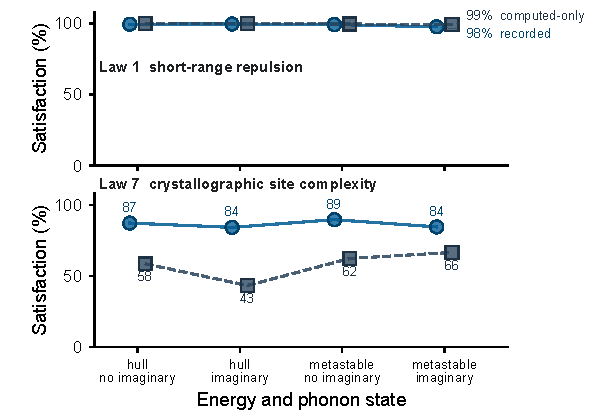
\includegraphics[width=0.72\textwidth]{figs/figS22_energy_phonon_record.pdf}
  \caption[Energy, phonons and experimental record]{\textbf{PRIS satisfaction across
  energy, phonon and experimental-record classes.} The horizontal axis crosses on-hull or
  metastable status with the absence or presence of imaginary phonon modes. The upper and
  lower profiles show satisfaction of Law~1 and Law~7, respectively. Solid blue circles
  denote experimentally recorded structures, and dashed grey squares denote computed-only
  structures. Connecting lines guide the eye.}
  \label{sifig:energy-phonon-record}
\end{figure}

\begin{figure}[!htbp]
  \centering
  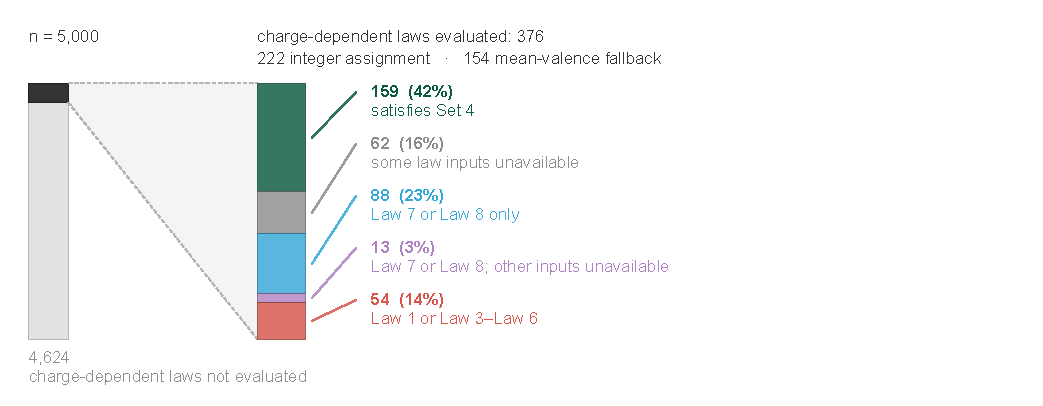
\includegraphics[width=\textwidth]{figs/figS23_charge_coverage.pdf}
  \caption[Coverage of charge-dependent PRIS laws in GNoME]{\textbf{Coverage of
  charge-dependent PRIS laws in GNoME.} Flow of the random GNoME sample through
  formal-charge assignment and the charge-dependent laws. The evaluable branch is divided by
  charge-assignment route and then by Set~4 outcome and violated mechanism. Structures without a
  formal-charge assignment are outside the evaluable domain of the charge-dependent laws and
  are not classified as satisfying or failing them.}
  \label{sifig:charge-coverage}
\end{figure}

\begin{figure}[!htbp]
  \centering
  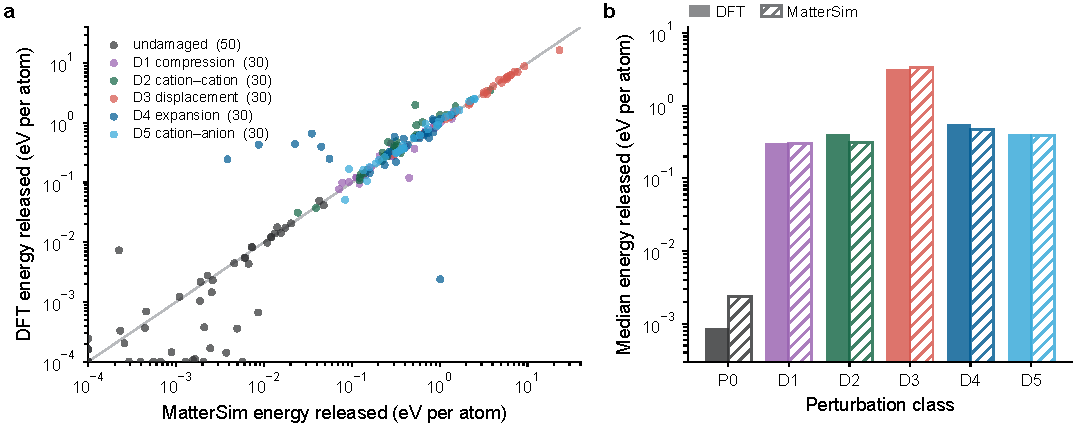
\includegraphics[width=\textwidth]{figs/figS24_dft_e3_paired.pdf}
  \caption[Machine-learned relaxation energies against first principles]{\textbf{The
  machine-learned potential against first principles on identical cells.}
  \textbf{a},~Energy released on relaxation for 200 cells. The damaged cohort contains
  thirty discovery-split experimental parents with each of five perturbations applied. The
  undamaged cohort contains fifty parents, including twenty GNoME entries. DFT and
  MatterSim evaluated the same geometries under the same frozen-cell protocol and have a
  Spearman rank correlation of 0.953. Points at the axis limits denote cells for which both
  methods give a release below the plotted floor. \textbf{b},~The same comparison resolved
  by perturbation class, which exposes any class-specific disagreement. Filled bars show
  DFT medians, and hatched bars show MatterSim medians.}
  \label{sifig:dft-e3-paired}
\end{figure}

\begin{figure}[!htbp]
  \centering
  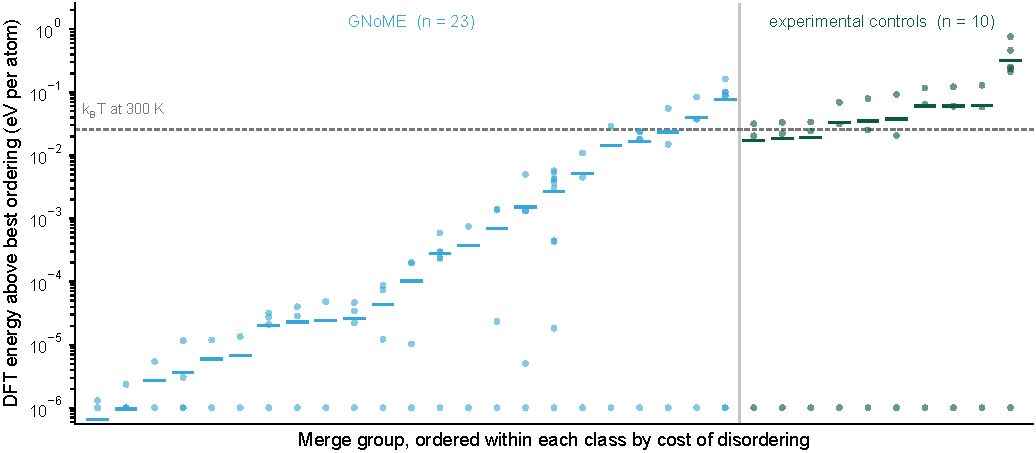
\includegraphics[width=\textwidth]{figs/figS25_dft_e2_ordering.pdf}
  \caption[Ordering energies behind the GNoME attribution]{\textbf{Ordering energies
  behind the chemical-label attribution.} For each merge group, every symmetry-distinct
  ordering of its mergeable species was relaxed with DFT. Points show each ordering's
  energy above the lowest-energy ordering in that group. The horizontal bar shows the cost
  of leaving that ordering for a random one, and groups are sorted within each class by
  this cost. The dashed line is $k_\mathrm{B}T$ at 300\,K. The GNoME groups have a median
  disordering energy of 0.00010\,eV per atom. The experimental controls have a median of
  0.03642\,eV per atom, which is 358 times larger. No control falls below 300\,K on this
  measure, whereas 18 of 23 GNoME groups do. An ordering that costs less than room
  temperature to scramble describes a solid solution rather than an ordered crystal.
  Supplementary Section~\ref{note:dft} explains which quantity distinguishes order from
  disorder.}
  \label{sifig:dft-e2-ordering}
\end{figure}

\subsection{Most thresholds selected on discovery data give similar verdicts on held-out data}

Every numeric threshold in the eight laws corresponds to a stated percentile of its quantity
in the experimental-structure discovery distribution. We tested threshold stability by
re-deriving each constant at the same percentile on the held-out split. We then measured
the shift in each threshold and the fraction of verdicts that changed when the re-derived
value replaced the original.

\begin{center}
\small
\setlength{\tabcolsep}{3pt}
\begin{tabular}{lccccc}
\hline
threshold & original & percentile & held-out & experimental flips & damaged flips \\
\hline
Law~1 $\tau$ & 0.735 & 1.0\% & 0.745 & 0.19\% & 1.6\% \\
Law~1 $\tau$ (tight) & 0.804 & 3.0\% & 0.809 & 0.17\% & 1.2\% \\
Law~2 ceiling & 1.05 & 99.4\% (ionic) & 1.043 & 0.12\% & 0.11\% \\
Law~3 ceiling & 1.081 & 96.7\% (conditional) & 1.065 & 0.64\% & 0.54\% \\
Law~4 range & 31.45 & 99.5\% & 26.4 & 0.25\% & 5.0\% \\
Law~5 max & 15.17 & 99.5\% & 3.9 & 0.33\% & 7.8\% \\
Law~7 distinct sites & 2/3 & 91.6\% & 3/4 & 2.9\% & 3.2\% \\
Law~8 deviation & 0.7143 & 96.0\% & 0.7143 & 0.00\% & 0.00\% \\
\hline
\end{tabular}
\end{center}

The contact, packing and valence
thresholds move by at most 1.5\% of their values. Law~8
returns at the same grid point. The two electrostatic thresholds lie in sparsely populated
tails, so their numerical values move substantially. For example, the maximum-site-energy
threshold changes from 15 to 4\,eV. Yet these changes flip fewer than 0.4\% of
experimental-structure verdicts. For deliberately permissive extreme-value laws, the
verdict is therefore more stable across splits than the exact decimal threshold. Law~7
lies on a discrete grid of small-integer fractions, so its selected percentile threshold
changes from 2/3 to 3/4.

\subsection{Law evaluation is negligible beside DFT relaxation}

We benchmarked the implementation on one CPU core of the analysis machine. Each
measurement used a rock-salt supercell and a new Python process. Law~1 requires one
neighbour scan and one radius lookup. It costs 0.05\,ms for an 8-atom cell, 1.0\,ms for
64 atoms and 10.7\,ms for 216 atoms.

The full eight-law reference implementation calls neighbour assignment three times. It
costs 58\,ms, 512\,ms and 2.4\,s on the same cells, while charge assignment adds
0.1--0.3\,ms. These are measured implementation costs rather than algorithmic limits.
Computing the same quantities from one cached neighbour list would be approximately three
times faster.

For generative-model outputs containing 6--20 atoms per cell, Law~1 screens a queue of
10{,}000 structures in under one second. The unoptimised eight-law implementation takes
approximately ten minutes. A literature estimate of 100 CPU hours per structure projects
approximately $10^6$ CPU hours for 10{,}000 DFT relaxations (main-text ref.~1). This is an
order-of-magnitude projection, not a DFT measurement on the screened queue.

\section{Shared evaluation procedure across pre-registered analyses}\label{note:s19}

\textbf{Split details.} The pre-registered split assigned 22{,}925, 9{,}634 and
5{,}748 structures to the discovery, held-out and reserve partitions, respectively. The
analysis populations are the subsets with a charge assignment and all required features
(Section S2). Assignment hashes structure identifiers rather than compositions. Different
structures of the same composition can therefore occupy different partitions. Agreement
between splits measures consistency for this random split, not performance on unseen
chemistries. The composition-unseen sensitivity analysis in Section~S8 restricts the frozen
evaluation to reduced compositions absent from discovery, but remains a subgroup of the
existing held-out partition rather than a new external cohort. The omitted-damage-type tests
provide evidence beyond the damage classes used for selection.

\textbf{Protocol of the fitted synthesis score.} PSS (Section S15) was run under a written
pre-registration fixed before fitting and archived with a time stamp and cryptographic
hash. The model is an antisymmetric pairwise logistic score without an intercept. Missing
features are filled with development-set medians, and all features are standardised using
development-set statistics only. Pairs are weighted so that each composition contributes
equally. Greedy
forward selection uses grouped five-fold cross-validation, a minimum decision rate of
0.99 and a minimum required gain of 0.002, with at most eight terms.

A seeded hash split the 1{,}508 composition groups into 919 development groups and 589
held-out groups. A script that refuses a second run evaluated the held-out set exactly
once. For full-pool transfer, the fixed coefficients and preprocessing statistics were
applied without refitting. The code archive contains all coefficients, preprocessing
statistics, criterion verdicts and evaluation logs.

\textbf{The Set~4 analysis.} The Set~4 analysis (Section S17) fixed its
procedure before the augmented features existed. Set~3 was first reproduced to four
decimal places on both splits, and damaged structures were recreated from the original
seeds. Greedy selection maximised combined damage detection while requiring satisfaction
of at least 0.81 among experimental discovery structures. Candidate thresholds came from
a fixed percentile grid. The held-out split was evaluated once. Omitted-damage variants
refitted only the additions above the fixed Set~3 base.

The PSS confidence breakdown in main-text Fig.~4e was examined after held-out evaluation.
It is identified wherever quoted as an exploratory ordering analysis.

\section{Pre-registered first-principles tests of four learned quantities}\label{note:dft}

Four quantities used in the main text were initially learned from data or machine-learning
predictions rather than calculated directly with DFT. They are the contact thresholds of Law~1 and Law~2, the artificial chemical ordering behind GNoME's low-symmetry excess,
the damage-severity
scale predicted by a machine-learned potential, and the predicted property used to select
the design queue. Each quantity was re-derived with plane-wave DFT under a protocol frozen
before any calculation was submitted. The \texttt{dft/} directory of the source repository
contains the pre-registration, task packages, extraction and analysis.

\paragraph{Protocol.} Calculations used VASP 6.3.0 with PBE PAW potentials recommended by
\texttt{MPRelaxSet}. The plane-wave cutoff was
$\max(520\,\mathrm{eV}, 1.3\max\mathrm{ENMAX})$. Static calculations used an explicitly
written $\Gamma$-centred mesh at $0.22\,\text{\AA}^{-1}$, \texttt{EDIFF}
$=10^{-6}$\,eV and tetrahedron smearing. Cell relaxations used \texttt{ISIF}~$=3$.
Constant-volume points on the energy--volume curves used \texttt{ISIF}~$=4$. The campaign
comprised 1{,}917 tasks and approximately 344 node-hours.

\paragraph{What each experiment measures.} Five experiments answer four questions. Two
experiments map the contact landscape and provide its hard-potential control
(Fig.~\ref{sifig:dft-e1-landscape}a,b). The remaining three measure ordering energies
(Fig.~\ref{sifig:dft-e2-ordering}), test machine-learning predictions of damage severity
(Fig.~\ref{sifig:dft-e3-paired}) and evaluate the property screen
(Fig.~\ref{sifig:dft-e4-bulk}). The ordering and property tests require distinct evaluation
quantities, defined below.

For the ordering analysis, the energy above the best ordering tests whether the release
selected the ground state. It does not determine whether the compound remains ordered.
Thirteen of the 23 GNoME entries lie exactly at the minimum, which supports the released
ground-state assignment. Order versus disorder is instead decided by the cost of leaving
the best ordering for a random one. On this measure, no experimental control falls below
300\,K, whereas 18 of 23 GNoME groups do. Figure~\ref{sifig:dft-e2-ordering} shows both
quantities.

For the property screen, the 400\,GPa target was set using machine-learning predictions of
the bulk modulus. The DFT value is a median 0.940 times the predicted value, showing that
the predictions run high. An unscaled absolute threshold would therefore test model
calibration rather than candidate selection. Accordingly, only 0.7\% of the candidates
predicted to have high bulk modulus exceed an unscaled 400\,GPa under DFT. The correlation
between predicted and DFT values is $r=0.769$. Thus, ranking rather than absolute scale
transfers between the model and DFT, and the selection holds at the rescaled threshold
(Fig.~\ref{sifig:dft-e4-bulk}).

\paragraph{The relaxed design candidates, and what relaxing them changes.} The 260
candidates whose bulk moduli were computed are provided as Supplementary Data, with one CIF
per candidate. The index reports composition, PSS and the computed modulus. It also reports
space group and distinct-site fraction before and after relaxation.

Conditioning the generator on a bulk modulus above 400\,GPa concentrates its output in a
narrow region of the periodic table. Only eleven elements appear, and Os, Ir and Re account
for almost every candidate (Fig.~\ref{sifig:dft-e4-composition}a). Relaxation also changes
the symmetry used for Law~7 assessment. On the generated coordinates, 61 of the 260
candidates satisfy the Law~7 threshold. After relaxation, 113 satisfy it, and none moves in the
opposite direction. This one-way change occurs because relaxation merges sites but does not
split them.

The shift is concentrated among candidates that the screen retained. After relaxation,
57.9\% of the high-property candidates satisfy Law~7, compared with 11.7\% of the removed
candidates. PSS calculated from unrelaxed coordinates therefore anticipates which cells
subsequently relax into law-satisfying structures. Because relaxation data were absent from
PSS construction, this provides an independent check of the screen.

\paragraph{Sensitivity of the fitted moduli.} The Birch--Murnaghan fit has four parameters,
so a five-point energy--volume curve leaves one degree of freedom. We tested sensitivity by
dropping one point from every candidate with five converged values. The fitted modulus
shifts by a median of 0.05\,GPa. This shift is three orders of magnitude smaller than the
difference between the median moduli of retained and screened candidates.


\begingroup
\linespread{1.25}\selectfont
\bibliography{refs}
\endgroup

\end{document}
